% !TEX TS-program = pdflatex
% !TEX encoding = UTF-8 Unicode

% This is a simple template for a LaTeX document using the "article" class.
% See "book", "report", "letter" for other types of document.

\documentclass[11pt]{article} % use larger type; default would be 10pt

\usepackage[utf8]{inputenc} % set input encoding (not needed with XeLaTeX)

%%% Examples of Article customizations
% These packages are optional, depending whether you want the features they provide.
% See the LaTeX Companion or other references for full information.

%%% PAGE DIMENSIONS
\usepackage{geometry} % to change the page dimensions
\geometry{a4paper} % or letterpaper (US) or a5paper or....
\geometry{margin=20mm} % for example, change the margins to 2 inches all round
% \geometry{landscape} % set up the page for landscape
%   read geometry.pdf for detailed page layout information
\setlength{\parindent}{0em}
\setlength{\parskip}{2em}
\usepackage{graphicx} % support the \includegraphics command and options

% \usepackage[parfill]{parskip} % Activate to begin paragraphs with an empty line rather than an indent

%%% PACKAGES
\usepackage{booktabs} % for much better looking tables
\usepackage{array} % for better arrays (eg matrices) in maths
\usepackage{paralist} % very flexible & customisable lists (eg. enumerate/itemize, etc.)
\usepackage{verbatim} % adds environment for commenting out blocks of text & for better verbatim
%\usepackage{subfig} % make it possible to include more than one captioned figure/table in a single float
\usepackage{subcaption} % make it possible to include more than one captioned figure/table in a single float
% These packages are all incorporated in the memoir class to one degree or another...

%%% HEADERS & FOOTERS
\usepackage{fancyhdr} % This should be set AFTER setting up the page geometry
\pagestyle{fancy} % options: empty , plain , fancy
\renewcommand{\headrulewidth}{0pt} % customise the layout...
\lhead{}\chead{}\rhead{}
\lfoot{}\cfoot{\thepage}\rfoot{}

%%% SECTION TITLE APPEARANCE
\usepackage{sectsty}
\allsectionsfont{\sffamily\mdseries\upshape} % (See the fntguide.pdf for font help)
% (This matches ConTeXt defaults)

%%% ToC (table of contents) APPEARANCE
\usepackage[nottoc,section, numbib]{tocbibind} % Put the bibliography in the ToC
\usepackage[titles]{tocloft} % Alter the style of the Table of Contents
\renewcommand{\cftsecfont}{\rmfamily\mdseries\upshape}
\renewcommand{\cftsecpagefont}{\rmfamily\mdseries\upshape} % No bold!
%%% END Article customizations
\graphicspath{ {./resources/} }
\usepackage[hidelinks]{hyperref}
\usepackage{amsmath}
\usepackage{amsfonts}
\hypersetup{
    colorlinks=true,
    citecolor=[RGB]{0,0,200},
    linkcolor=[RGB]{128,0,0},
    filecolor=magenta,      
    urlcolor=cyan,
    pdftitle={Driftworld},
    pdfauthor={Adalbert Delong},
    }

\title{Driftworld Tectonics 1.0: an overview}
\author{Adalbert Delong}
\date{31th July 2022}

\begin{document}
\maketitle
%\section*{Abstract}
Driftworld Tectonics is a project written for Unity editor, used to create basic forms of planets. It utilizes ideas and methods described in an article by Yann Cortial et al. in 2019 \cite{cortial}. Planets are created by~reading basic template topology, performing a simplified tectonic simulation of the planet's crust and~then exporting the raw data to customized binary files. Users can display various overlays of the~planet during the simulation, as well as see the surface elevation mesh.\par
This documentation describes some basic theoretical framework, details of the simulation and the implementation. Hopefully it can be of use to anyone interested in this topic, who either just wants to play around with Driftworld or build their own projects.\par
Project Driftworld is licensed under a \href{https://creativecommons.org/licenses/by/4.0/}{Creative Commons Attribution 4.0 International License}.
\section*{Acknowledgements}

I would like to thank Dr. Yann Cortial of the National Institute of Applied Sciences of Lyon for discussing his article. His answers to my various inquiries helped me decide the scope and form of Driftworld. I would also like to thank Dr. Daniel Meister of AMD Japan Co. Ltd. for his comments on the use of bounding volume hiearchy algorithms. Driftworld implements a part of an algorithm described in one of his publications \cite{meister}. More thanks to \href{https://www.prowaretech.com}{PROWAREtech} for allowing me to include an adapted version of an example implementation of Mersenne Twister random number generator in the project.

I would like to thank Ben Golus for his help with UV texture mapping and his advice on texturing. %href??

Special thanks to my friends Vilém and Matyáš and other members of our Discord server for discussing ideas and for their feedback.

The project was created using Unity Editor, lately in its version 2021.3.1f1. The C\# code is kept in a~MS Visual Studio Community 2022 project, image materials come from Unity Editor screenshots, Geogebra projects and Blender. Documentation uses \LaTeX\hspace*{0.3em}in its TeX Live implementation.
\section*{Disclaimer}

Over the past two years, Driftworld evolved both in terms of ideas and terms of implementation. The absolute majority of concepts beyond mathematics were completely new to me when the project started, so the code changed often and many times was almost completely rewritten as I learned. Some older parts remained which can cause a correct impression of inhomogeneity. I do not claim the implementation is flawless and although a lot of the shaky cases were accounted for, some unforseen mistakes may and probably do remain.

I would like to ask anyone using the project to tolerate possible mistakes. There is more work to be done and I would be grateful for feedback.

Thank you for your consideration.
\newpage
\tableofcontents
\newpage
\section{Introduction}
\label{sec:introduction}
Driftworld Tectonics is a Unity project created for use in the Unity editor. The entirety of interactivity is within the editor GUI and the project has no meaningful executable scene. Any feedback is in a~console log and the state of the planet is observed within the static scene rendering. This is the most obvious difference from the implementation in the original article from which Driftworld draws inspiration - simulation described in the article offers interactivity while the simulation is running \cite{cortial}.

The workflow follows Cortial et al. in a lot of details, although experience and chosen software tools pose several restrictions. At first a Delaunay triangulation mesh is imported from prepared binary files. Then a set of tectonic plates is created by partitioning said mesh. The planet evolution is performed in repeated tectonic steps. Every step deals with plate subduction, possible continental collision, new crust creation because of diverging ocean plates, slab pull due to subduction influence, erosion and crust damping, and finally, rifting plates. At any time the current state can be saved as a binary file for further use. This follows the original article \cite{cortial}. Driftworld, however, differs in two rather important steps: continental collisions are always plate-wide and plate rifting follows somewhat different probability mechanics. This is mainly for fine-tuning and can change in future updates, as these changes further simplify an already simplified model and were done as a saving grace from implementation difficulties.

The output of Driftworld is binary planet data with varying resolution of sphere sampling. Provided data are: crust age, elevation, plate assignment, crust thickness and orogeny. The binary file keeps the original topology for easier manipulation. The user can also at any time export the current texture overlay as a PNG image.

This documentation serves both as a user's manual and a quick introduction into the problematic. Section \ref{sec:geometry} defines basic terms, mathematical objects and their properties. Section \ref{sec:tectonicmodel} follows with details of the used simplified tectonic model. The actual implementation with neccessary details and context are discussed in the section \ref{sec:implementation}. As an important part, performance of the simulation and related issues are the topic of section \ref{sec:performance}. We conclude the status quo of the project in section \ref{sec:conclusion}.

\subsection{Motivation}
\label{subsec:motivation}
Procedural terrain generation is an important part for a number of computer games \cite{generatedgames}. Usually, these games employ random generators to increase variety on a theme, such as a map layout. Indeed, in my subjective opinion a~player's experience is greatly enriched by variety, especially in the game environment. This comes with an apparent caveat that purely procedural generation may lack the sense of creativity, leading to mundanely repeating patterns \cite{daggerfall}. 

With the onset of newer technologies (e. g. increased GPU power), we are able to perform more computationally-intensive tasks. When it comes to the terrain generation, even a regular user without access to high-tier hardware can try more sophisticated alternatives to simpler algorithms. Arguably, more realistic worlds bring the feeling of familiarity to the experience. If we can create a~more realistic, yet still random map/world/neighbourhood, the possibilities are endless.
\newpage
Following thoughts are purely my personal view. As a life-long video games fan, I have always gravitated towards story-telling games, especially those taking place in an open world. Among these, I'd like to mention Baldur's Gate series, The Elder Scrolls series, Might \& Magic series, Fallout 4 and Mass Effect series. At the same time, I have been also drawn to grand building games taking place in complex worlds. Transport Tycoon or Caesar III and its modern re-implementation Augustus \cite{augustus} were a heavy influence, lately Factorio or Rimworld. Rimworld stands apart in its uniqueness, as it can be understood rather as a story generator than a game \cite{rimworld}. In large part, the idea of Driftworld came from the works of J. R. R. Tolkien and watching the 1997-2007 Stargate series - the series' take on mythology context in human societies in particular.

Epic stories build on cohesion. In this regard, countless debates take place about details. It takes a~great deal of time to create viable environment to match an idea for a story, especially if that story is told over long periods of time. Driftworld aspires to one thing: help create a platform in which stories can take place. First step is this project -- to create a rough map. 

\section{Spherical geometry \& topology}
\label{sec:geometry}
The most fundamental object with which Driftworld Tectonics works is a mesh of a sphere in the 3D Euclidean space. For simplicity, we assume the sphere is a unit sphere centered on the origin unless stated otherwise. Because of the spherical nature of the project, several (arguably) uncommon mathematical concepts are described in this section -- such as vertex sampling, triangulation, transformations or bounding volume hiearchies. Although the text follows almost a textbook-like mathematical structure, a lot of the formulations and conclusions lack correct proof. Some reasoning is made to carry a~point, but meticulous readers are left to their own devices.
\subsection{Unity coordinate system}
\label{subsec:unitycoords}
Unity uses a left-handed coordinate system with the \textit{x} axis pointing to the right, \textit{y} axis pointing upwards and \textit{z} axis pointing forward (see Figure \ref{fig:unity-coordinate}). This is reflected in the scenes -- nevertheless, the mathematical expressions of vectors themselves are identical to a standard right-handed coordinate system, i. e. the following holds for the basis:
$$\mathbf{e}_x \times \mathbf{e}_y = \mathbf{e}_z$$
All implementations must be aware of the fact that the cross product expressions do not distinguish between right-handed and left-handed. It is simply a matter of axes display, where visually 'switching' axes \textit{y} and \textit{z} alternates between left-handedness and right-handedness. In the left-handed coordinate system, right-hand rule of cross product shows the inverse final direction of the cross product.
\begin{figure}[ht]
\centering
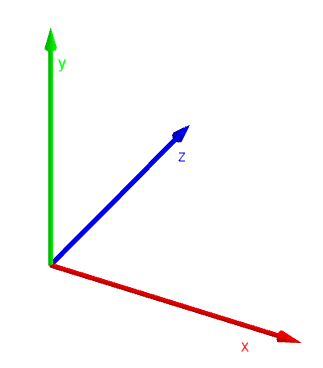
\includegraphics[height=7cm]{unity-axes.png}
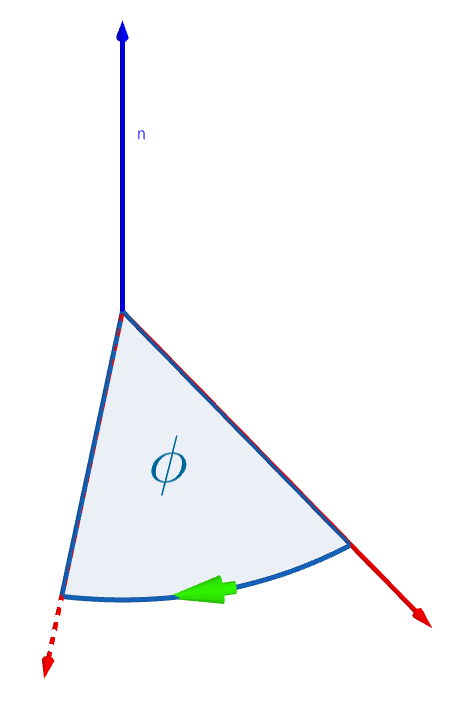
\includegraphics[height=7cm]{unity-rotation.png}
\caption{Unity coordinate system}
\label{fig:unity-coordinate}
\end{figure}

There are several ways to rotate points, vectors or whole transformations. For clarity, let us assume a 3-dimensional vector $\mathbf{u}$ that is to be rotated. We define a rotation unit vector $\mathbf{n}$ and an angle $\phi$ by which we rotate $\mathbf{u}$ so that $\mathbf{u}$ rotates by $\phi$ within a plane to which $\mathbf{n}$ is normal. We also assume that the rotation plane passes through the origin. Then from the perspective of a sundial (with $\mathbf{n}$ being the gnomon) $\mathbf{u}$ rotates \textit{clockwise} for positive $\phi$ (Figure \ref{fig:unity-coordinate}). This holds for all relative rotations.

\subsection{Sectional planes and great circles}
Sphere can have any number of sectional planes, i. e. planes that have some non-empty intersection with the sphere. Planes passing the center of the sphere will be called \textit{sectional central planes} (Figure \ref{fig:sectional-plane}). Any sectional central plane $\rho$ is characterized by some non-zero normal vector $\textbf{n}_\rho$ and for any point on the plane represented by their position vector $\mathbf{x}$ it holds that
$$\mathbf{n}_\rho\cdot\mathbf{x}=0$$
This is synonymous to the fact that any vector lying within a plane passing the origin is perpendicular to the normal vector of the plane. The dot product on the left side of the equality is also important because given a specific normal vector we can decide on which side is any vector $\mathbf{x}$ \textit{outside} the plane -- simply take the sign of the dot product, vector on the side of the normal vector will result in a positive dot product value with $\mathbf{n}_\rho$, negative otherwise.

An important object on the surface of a sphere is a great circle. It is any circle that shares its center and radius with the sphere (Figure \ref{fig:great-circle}). It is also the intersection of a plane passing the center of the sphere with its surface.
\begin{figure}[ht]
\centering
\begin{subfigure}{7cm}
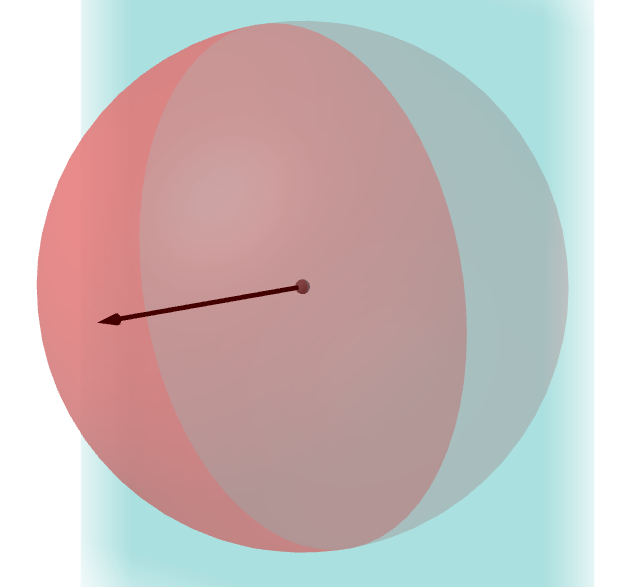
\includegraphics[height=6cm]{sectional-plane.png}
\caption{central plane}
\label{fig:sectional-plane}
\end{subfigure}
\begin{subfigure}{7cm}
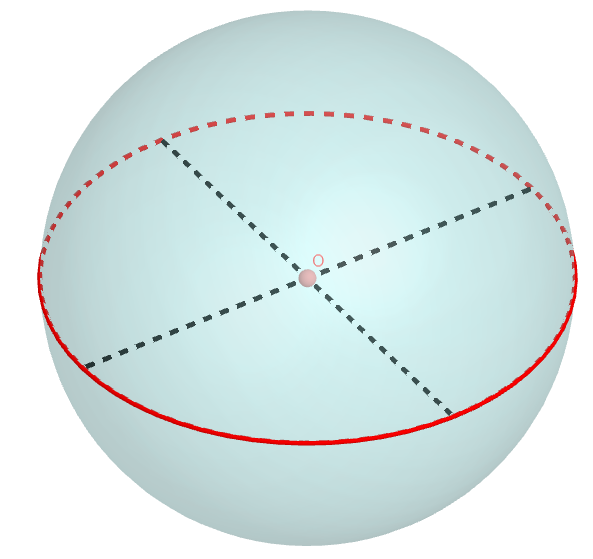
\includegraphics[height=6cm]{great-circle.png}
\caption{great circle}
\label{fig:great-circle}
\end{subfigure}
\caption{Sphere section by plane}
\label{fig:sectional-objects}
\end{figure}

\subsection{Spherical triangles}
Any three points on the surface of a sphere that do not lie on a single great circle form a~\textit{spherical triangle} (Figure \ref{fig:spherical-triangle}). This is the fundamental concept behind many of the computations in the project. However, strictly speaking, there are two triangles defined by such three points. The closure of the complement of any spherical triangle with respect to the sphere surface is also a spherical triangle, albeit one of the two is unintuitive as it is larger than half of the sphere surface area. To get around this, we construct somewhat narrower class of spherical triangles so that any three valid points define a triangle unambiguously.

\begin{figure}[ht]
\centering
\begin{subfigure}{8cm}
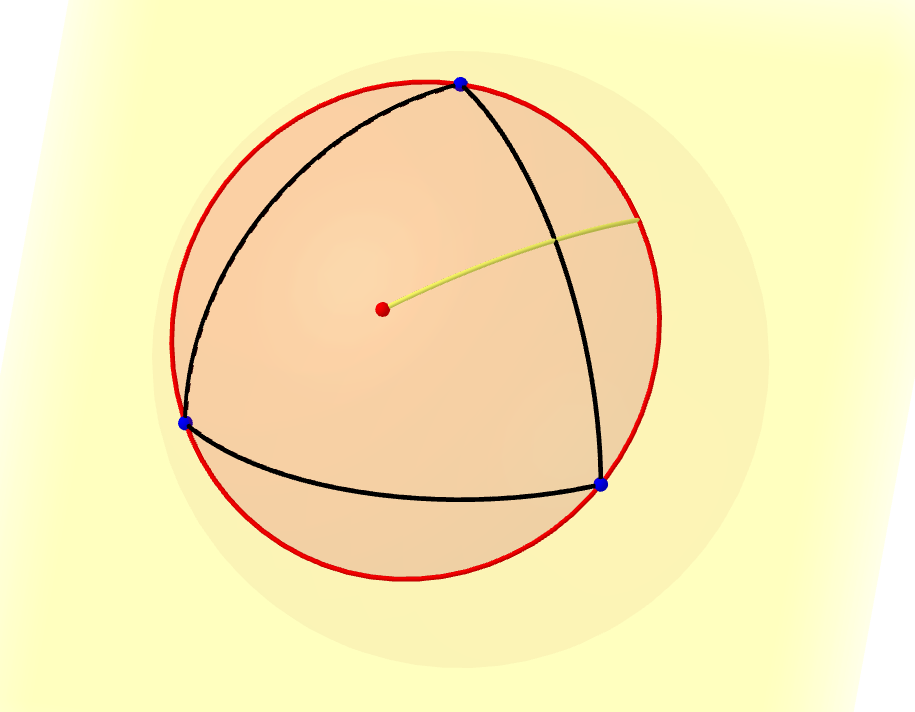
\includegraphics[height=6cm]{triangle-circumcircle.png}
\caption{with sectional plane and circumcircle}
\label{fig:triangle-circumcircle}
\end{subfigure}
\begin{subfigure}{8cm}
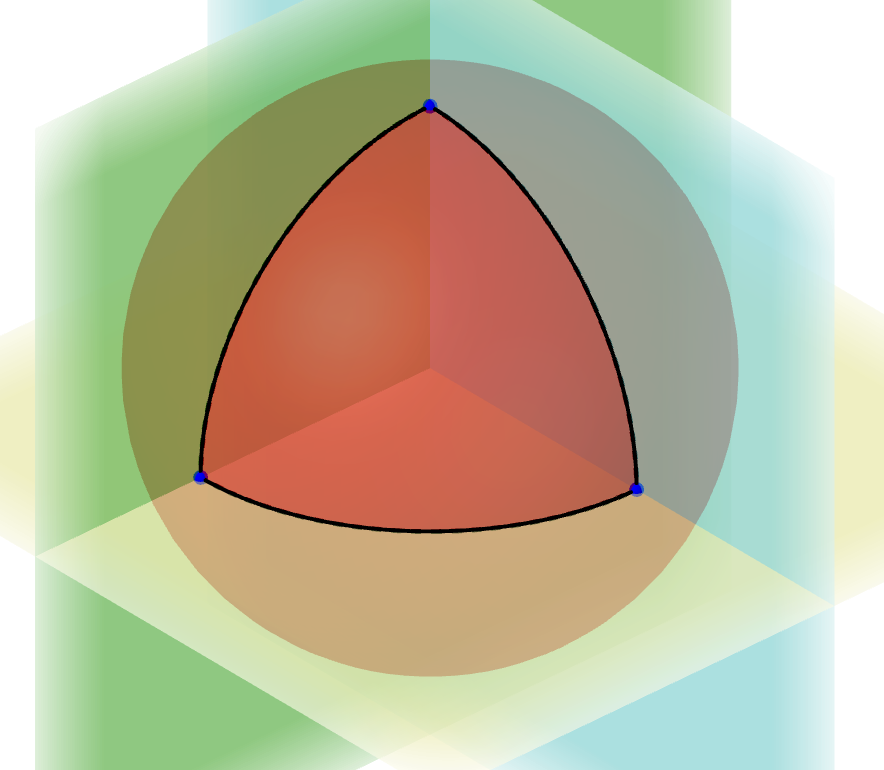
\includegraphics[height=6cm]{triangle.png}
\caption{planes intersections}
\label{fig:spherical-triangle-visual}
\end{subfigure}
\caption{Spherical triangle}
\label{fig:spherical-triangle}
\end{figure}

 We denote the surface of a unit sphere $\mathcal{S} =  \{\mathbf{x} \in \mathbb{R}^3: ||\mathbf{x}||=1\}$. Given a triplet of three linearly independent point vectors $(\mathbf{a},\mathbf{b},\mathbf{c})\in \mathcal{S}\times\mathcal{S}\times\mathcal{S}$ (called \textit{vertices})\footnote{Linear independence of unit vectors is equivalent to the condition that the vectors do not lie on a single great circle.}, we can construct a vector $\mathbf{n}_\lambda$ normal to some sectional plane $\lambda$ cutting off a spherical cap (Figure \ref{fig:sectional-plane}):
 $$\mathbf{n}_\lambda=(\mathbf{b} - \mathbf{a})\times(\mathbf{c} - \mathbf{a})$$
$$\forall\mathbf{x}\in\lambda: \mathbf{n}_\lambda\cdot\mathbf{x}+d_\lambda=0$$
We can calculate $d_\lambda$ by assigning e. g. $\mathbf{x}=\mathbf{a}$ and solving the plane equation with respect to $d_\lambda$, but that will not be neccessary. We impose a further requirement $\mathbf{n}_\lambda\cdot\mathbf{a}>0$. This is not always true, in which case it can be ensured by swapping any two vertices in the triplet and recalculating $\mathbf{n}_\lambda$. This means that all three vertices and their circumcenter are all 'on one side' of the sphere. In Unity coordinate system, this also means that for an outside observer, the vertices are oriented \textit{clockwise} on the sphere surface.

Spherical circumcircle $l$ is a set of points on a sphere that has constant spherical distance from a single point $\mathbf{c}_\mathcal{T}\in\mathcal{S}$ called \textit{circumcenter}. Equivalently, we can substitute dot product for distance:
$$\exists k\in\mathbb{R}:(\forall\mathbf{x}\in l:\mathbf{c}_\mathcal{T}\cdot\mathbf{x}=k)$$
Since $\mathbf{n}_\lambda\cdot\mathbf{a}=\mathbf{n}_\lambda\cdot\mathbf{b}=\mathbf{n}_\lambda\cdot\mathbf{c}>0$, we know that some scalar multiple of $\mathbf{n}_\lambda$ is the circumcenter for the vertices. In fact, there is only one possible circumcircle for all three vertices, which is the intersection $\mathcal{S}\cap\lambda$. We easily find the circumcenter and the circumradius $r_l$ as\footnote{We have to keep in mind that on a unit sphere, central angle and spherical distance are identical, barring formal dimension.}
$$\mathbf{c}_\mathcal{T}=\frac{\mathbf{n}_\lambda}{||\mathbf{n}_\lambda||}, r_l=\arccos(\mathbf{c}_\mathcal{T}\cdot\mathbf{a})$$

Previous reasoning allows us now to test if some point $\mathbf{x}\in\mathcal{S}$ is inside a spherical triangle $\mathcal{T}\subset\mathcal{S}$ with clockwise-oriented vertices $(\mathbf{a}, \mathbf{b}, \mathbf{c})$.
Geometrically speaking, a spherical triangle is a region bounded by three arcs of great circles \cite{palmer}. We calculate three normal vectors:
$$\mathbf{n}_{\rho}=\mathbf{a}\times\mathbf{b},$$
$$\mathbf{n}_{\sigma}=\mathbf{b}\times\mathbf{c},$$
$$\mathbf{n}_{\tau}=\mathbf{c}\times\mathbf{a}.$$
These vectors define planes $\rho, \sigma, \tau$ so that
$$\rho=\{\mathbf{x}\in\mathbb{R}^3:\mathbf{n}_{\rho}\cdot\mathbf{x}=0\}$$
$$\sigma=\{\mathbf{x}\in\mathbb{R}^3:\mathbf{n}_{\sigma}\cdot\mathbf{x}=0\}$$
$$\tau=\{\mathbf{x}\in\mathbb{R}^3:\mathbf{n}_{\tau}\cdot\mathbf{x}=0\}$$
intersections $\rho\cap\mathcal{S}, \sigma\cap\mathcal{S}, \tau\cap\mathcal{S}$ are then great circles that always pass two of the vertices. Because of this, each one is divided by them into two arcs. There is only one triplet of arcs connected by the vertices that forms a meaningful region boundary on $\mathcal{S}$ (Figure \ref{fig:spherical-triangle-visual}). There are two such regions but we already bypassed this problem by ensuring orientation. We test the point $\mathbf{x}$ against following condition:
$$\mathcal{T}=\{\mathbf{x}\in\mathcal{S}:\mathbf{n}_{\rho}\cdot\mathbf{x}\ge 0, \mathbf{n}_{\sigma}\cdot\mathbf{x}\ge 0, \mathbf{n}_{\tau}\cdot\mathbf{x}\ge 0\}$$
This simply tells us that $\mathbf{x}$ is inside the spherical triangle $\mathcal{T}$ when it is on the surface of the sphere and also on one specific side of all three planes $\rho, \sigma, \tau$. This definition does not encompass all possible spherical triangles on a sphere, but it allows us to properly test the properties of any triangles used in reasonable spherical meshes.
\subsection{Vertex sampling}
Because of memory restrictions, sphere surface data is represented as a set of sampled points. We can identify these points as position vectors $\mathbf{u}_i$ from the global origin to sample points, resulting in a~sequence $U=\left(\mathbf{u}_i\right)_{i=0}^{N-1}, \mathbf{u}_i \in \mathcal{S}$. Samples are therefore three-dimensional normalized vectors. Driftworld uses spherical Fibonacci sampling \cite{keinert}. To get the sequence $U$, another sequence $F=\left(\mathbf{f}_i\right)_{i=0}^{N-1}$ is first computed, using the following definition:
$$\mathbf{f}_i=(\phi_i, z_i), \phi_i \in \mathbb{R}, z_i \in \mathbb{R},$$
$$\phi_i = 2\pi\left[\frac{i}{\Phi}\right],$$
$$z_i = 1-\frac{2i+1}{N}.$$
$\left[x\right]$ denotes the fractional part of $x$, $\Phi$ is the golden ratio $\Phi=\frac{\sqrt{5}+1}{2}$. The values of $\mathbf{f}_i$ actually lie on a~spiral on the surface of a cylinder with the radius of 1 and the height of 2 \cite{keinert}. $U$ is finally obtained by mapping $\mathbf{f}_i$ values to $\mathcal{S}$:
$$\mathbf{u}_i = (\sin{(\arccos{(z_i)})}\cdot\cos{\phi_i}, z_i, \sin{(\arccos{(z_i)})}\cdot\sin{\phi_i})$$
Note that this mapping reflects Unity's axes orientation and the first and the last samples of $U$ do not fall exactly on the poles.
\subsection{Centroids, data values and barycentric interpolation}
Driftworld often makes computations for points inside sperical triangles - notably, it uses triangle centroids to evaluate triangle neighbours. Calculating these points is not a trivial procedure and although for a long time there have been methods to do so, it would be too resource-consuming when performed on a larger scale. To save computation time, we assume that all evaluated triangles are nearly planar, i. e. their \textit{triangle excess} is negligible (Legendre's Theorem\footnote{This theorem is also known as Saccheri-Legendre theorem.} \cite{todhunter}). We calculate the centroid of a triangle by simply normalizing the sum of its vertices (Figure \ref{fig:triangle-centroid}):
$$\mathbf{b}_\mathcal{T}=\frac{\mathbf{a} + \mathbf{b} + \mathbf{c}}{||\mathbf{a} + \mathbf{b} + \mathbf{c}||}$$
\begin{figure}[ht]
\centering
\begin{subfigure}{7cm}
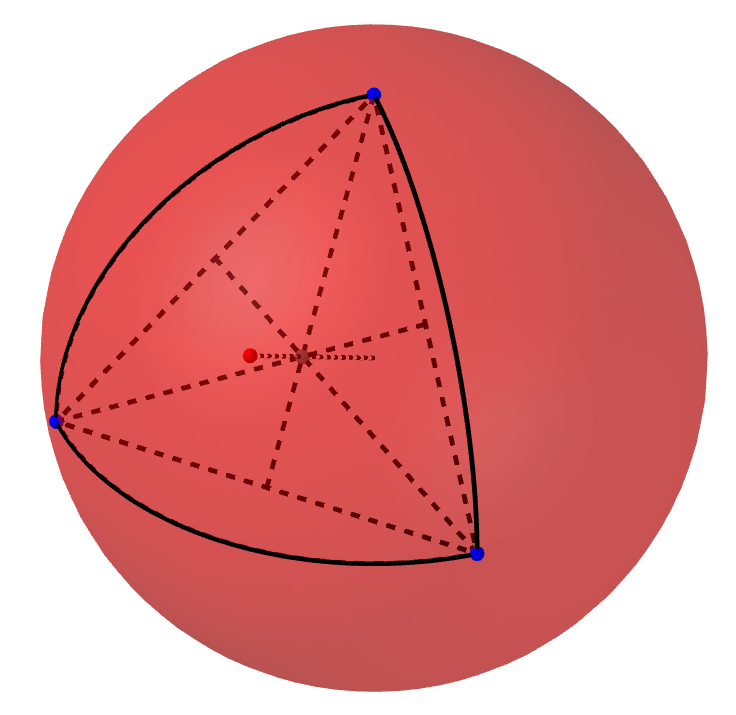
\includegraphics[height=6cm]{triangle-centroid.png}
\caption{sectional triangle centroid}
\label{fig:triangle-centroid}
\end{subfigure}
\hspace*{1cm}
\begin{subfigure}{7cm}
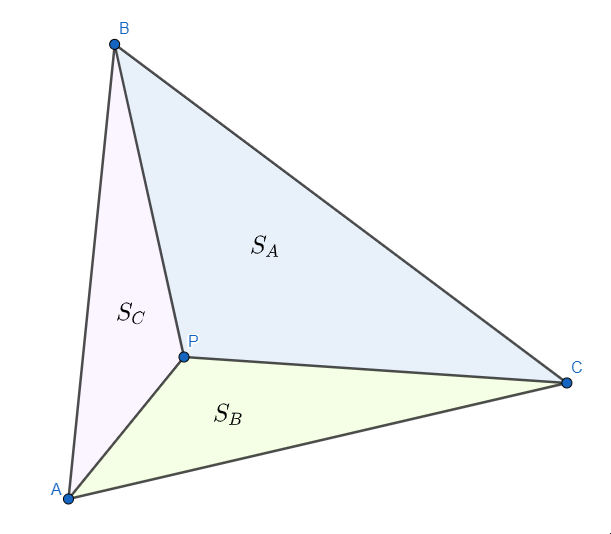
\includegraphics[height=6cm]{triangle-barycentric.png}
\caption{barycentric coordinates}
\label{fig:triangle-barycentric}
\end{subfigure}
\caption{Centroid geometry}
\label{fig:centroid-geometry}
\end{figure}

To store crust data, we must assign values to points on the sphere. These values may be of different types or have different meaning. Formally, we denote a sequence of arbitrary sets $C=\left(V_i\right)_{i=0}^{n-1}$, where $n$ is the number of different values assigned to a point and each $V_i$ is a specific of value. The system of all possible value combinations is then a cartesian product of these value sets:
$$V=\prod_{i=0}^{n-1}V_i$$
Stored data can then be defined as a map:
$$s: U\rightarrow V$$
$$s_i: U\rightarrow V_i$$
We store data only for sphere samples because of limited memory. Other values will be computed as needed using \textit{barycentric interpolation} \cite{scratchapixel}.\newpage

Now it comes to the following problem: how to compute values anywhere on $\mathcal{S}$? We are effectively looking for some domain extension, since $U\subset\mathcal{S}$:
$$s':\mathcal{S}\rightarrow V, \forall \mathbf{u}\in U:s'(\mathbf{u})=s(\mathbf{u})$$
$$s_i':\mathcal{S}\rightarrow V_i, \forall \mathbf{u}\in U:s_i'(\mathbf{u})=s_i(\mathbf{u})$$
Given some arbitrary point $\mathbf{x}\in\mathcal{S}$, we start with an assumption that $\mathbf{x}$ is found inside some spherical triangle $\mathcal{T}$ with negligible triangle excess and vertices $\{\mathbf{a}, \mathbf{b}, \mathbf{c}\} \subset U$ for which we already know the values of $s$. We would like $s'(\mathbf{x})$ to be computed 'fairly', i. e. the closer $\mathbf{x}$ is to some vertex, the more influence the vertex value should have on $s'(\mathbf{x})$. A good start might be in analogy with a political voting system based on area. If the population is homogeneous, any region vote is weighted by its area and transitionally, by its population.

Let $P$ be some point within a triangle $ABC$ (Figure \ref{fig:triangle-barycentric}). This point is represented by a point vector $\mathbf{p}\in\mathcal{S}$. As stated earlier, we assume all points lie nearly on the same plane. If we construct three triangles $PBC$, $APC$ and $APB$, the triangle $ABC$ will be divided into three regions, each corresponding to their oposite vertex of $ABC$. The closer $P$ is to any of the vertices, the larger the corresponding triangle area is. Total area sum of the three triangles is equal to the area of $ABC$. Therefore, we can use these triangle areas as weights for interpolating values at $P$ -- we only need to find the respective areas of $S_A, S_B, S_C$ and $S_{ABC}$. This can be done using cross product:
$$S_A=\frac{|(\mathbf{b}-\mathbf{p})\times(\mathbf{c}-\mathbf{p})|}{2}$$
$$S_B=\frac{|(\mathbf{c}-\mathbf{p})\times(\mathbf{a}-\mathbf{p})|}{2}$$
$$S_C=\frac{|(\mathbf{a}-\mathbf{p})\times(\mathbf{b}-\mathbf{p})|}{2}$$
$$S_{ABC}=\frac{|(\mathbf{b}-\mathbf{a})\times(\mathbf{c}-\mathbf{a})|}{2}$$
Since $S_A+S_B+S_C=S_{ABC}$, we can define normalized weights $u, v, w$ called \textit{barycentric coordinates}:
$$u=\frac{|(\mathbf{b}-\mathbf{p})\times(\mathbf{c}-\mathbf{p})|}{|(\mathbf{b}-\mathbf{a})\times(\mathbf{c}-\mathbf{a})|}$$
$$v=\frac{|(\mathbf{c}-\mathbf{p})\times(\mathbf{a}-\mathbf{p})|}{|(\mathbf{b}-\mathbf{a})\times(\mathbf{c}-\mathbf{a})|}$$
$$w=\frac{|(\mathbf{a}-\mathbf{p})\times(\mathbf{b}-\mathbf{p})|}{|(\mathbf{b}-\mathbf{a})\times(\mathbf{c}-\mathbf{a})|}$$
It is easy to confirm that $u+v+w=1$.

There are basically two types of values interpolated in the project -- real values and categories. Real value interpolation is straightforward:
$$s_i'(\mathbf{p})=us_i(\mathbf{a})+vs_i(\mathbf{b})+ws_i(\mathbf{c})$$
Categories are simply assigned to $\mathbf{p}$ according to the largest weight:
$$u=\mbox{max}(\{u,v,w\})\Rightarrow s_j'(\mathbf{p})=s_j(\mathbf{a})$$
$$v=\mbox{max}(\{u,v,w\})\Rightarrow s_j'(\mathbf{p})=s_j(\mathbf{b})$$
$$w=\mbox{max}(\{u,v,w\})\Rightarrow s_j'(\mathbf{p})=s_j(\mathbf{c})$$
This effectively draws a Voronoi map according to categories \cite{voronoi}.
\subsection{Spherical mesh and Delaunay triangulation}
There is a basic sphere mesh, provided by Unity (Figure \ref{fig:unity-mesh}). It is like a detailed cubic mesh, projected onto a sphere. However, for finer terrain details, a much more detailed mesh is needed, preferably with uniform triangles (Figure \ref{fig:delaunay-mesh}). Scaling the mesh detail is also important.

\begin{figure}[ht]
\centering
\begin{subfigure}{7cm}
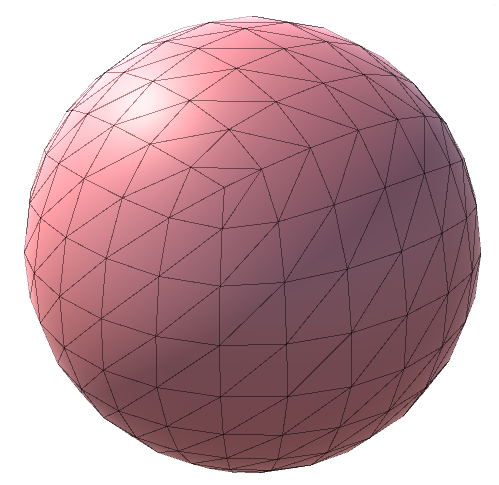
\includegraphics[height=7cm]{unity-mesh.png}
\caption{Unity sphere mesh}
\label{fig:unity-mesh}
\end{subfigure}
\hspace*{1cm}
\begin{subfigure}{7cm}
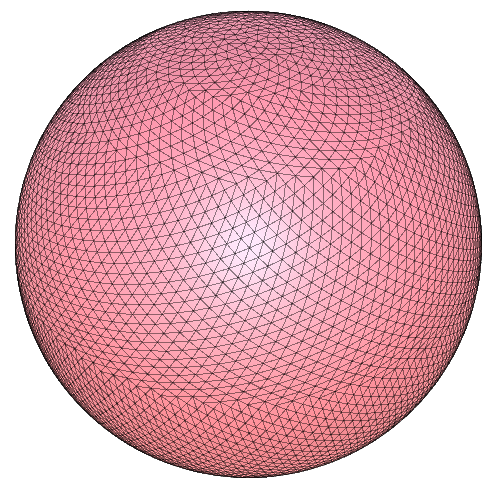
\includegraphics[height=7cm]{delaunay-mesh.png}
\caption{Delaunay mesh}
\label{fig:delaunay-mesh}
\end{subfigure}
\caption{Spherical meshes}
\label{fig:spherical-mesh}
\end{figure}
Definition and description of a 3D mesh is way beyond the scope and purpose of this document. In this context, it is simply an approximation of the sphere surface. All samples $U$ are vertices connected into triangles so that the whole sphere is covered by them without any gaps. For Driftworld, a set of prepared meshes is provided, created by \textit{Delaunay triangulation} \cite{delaunay}.

When interpolating surface data such as elevation, it is important that reasonable samples are used for the interpolation. Calculating elevation in a mountain range from a triangle with vertices too far apart may result in meaningless artifacts. Furthermore, the earlier mentioned requirement that the triangles are nearly planar would be undermined by extreme spherical triangles which exhibit considerable excess. It stands to reason that triangles used in the mesh should be as regular as possible. This is the goal and result of a Delaunay triangulation. There is a number of algorithms performing the triangulation on a plane \cite{knuth}. Since sphere has a closed mesh, an adaptation is needed.

Delaunay meshes for Driftworld use an algorithm which originally triangulates a set of random samples \cite{ma}. Because $U$ is ordered, the initial tetrahedron is somewhat difficult to construct, especially because of the requirements imposed on a spherical triangle -- in a large number of cases at least one triangle had a circumcircle larger than a great circle. For this reason, the initial structure was set to be a nearly regular octahedron with vertices assigned by a brute-force look-up. Other than that, the algorithm follows the article \cite{ma}.
\subsection{Bounding volume hiearchy}
\subsection{Collisions}


\section{Tectonic model}
\label{sec:tectonicmodel}
We now introduce the detailed description of the tectonic model used to create the planet crust. We discuss differences and similarities with respect to the original article and adapt the mechanisms to our unit sphere representation. Parameters that drive the model are summarized at the end of the section in Table \ref{tab:model-parameters-summary}. It should be stated that all parameters will be optimized for the number of vertex samples $N$ equal to 500,000.

The simplest description of the algorithm is that it creates some random crust partitioning into plates. These plates have randomized drifting parameters for moving. Then a certain number of tectonic steps is performed with a time step length $\delta t$ of 2 My and the result is a basic crust of the simulated planet. Between automated tectonic steps, user can force a few specific interactions (plate rifting, terrain smoothing) and change various global parameters to influence the simulation. The planet radius is set to $6370\mbox{ km}=6.37\mbox{ u}$.
\subsection{Workflow}
Basic crust is generated from a Delaunay triangulation of a unit sphere. The fresh crust is just a set of triangulated vertices, while each vertex is assigned some default crust data $h$. Each tectonic step consists of several substeps in a sequence. This sequence is firmly set because of implementation context and is depicted in Figure \ref{fig:tectonic-step-structure}. Short descriptions for the substeps follow.
\begin{figure}[ht]
\centering
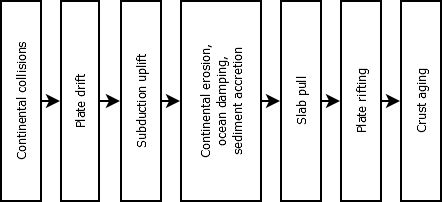
\includegraphics[width=12cm]{tectonic-step-structure.png}
\caption{Tectonic step structure}
\label{fig:tectonic-step-structure}
\end{figure}
\begin{itemize}[\label={}]
\item[\textbf{Continental collisions}] If the plate drift would result in an overlap of two different continental (above sea level) areas of crust belonging to different plates, a continental collision is triggered, resulting in a~massive uplift of the lighter plate. The two plates in question are then merged into one. This is different from the orignal algorithm, which only attaches connected continental areas, called \textit{terranes}.
\item[\textbf{Plate drift}] Rotation transform of each plate along the sphere surface is updated by its respective angular speed.
\item[\textbf{Subduction uplift}] Overlapping areas of different plates cause uplift in the lighter plates. This process is known as \textit{subduction}. Note that overlapping continental areas have already been dealt with so this case should never occur during this step.
\item[\textbf{Continental erosion, ocean damping, sediment accretion}] This step updates elevation values to simulate erosion of crust above sea level, lowering of the ocean bottom for underwater crust and sediment accretion for the ocean crust below average ocean depth. This is questionable, as the original algorithm probably detects trench area for sediment filling.
\item[\textbf{Slab pull}] Subducting parts of plates tend to pull the plate towards them, altering the surface rotation. All vertices in subduction zones contribute to the rotation vectors of their plates.
\item[\textbf{Plate rifting}] Every tectonic step the largest plate has a chance to rift apart. Along some random linear border within the plate the vertices are assigned to two new plates with diverging velocities.
\item[\textbf{Crust aging}] Age of every crust vertex is updated by the length of the tectonic step.
\end{itemize}
\subsection{Crust \& plates}
The crust is defined as a set of surface vertices $U$, obtained by Fibonacci sampling. Its size is the number of samples $N$. Each vertex $\mathbf{u}_i\in U$ is assigned crust point data $h_i$. The tectonic plate system is an~equivalence system $\mathcal{P}$ of $U$ (so that every crust point belongs exactly to one plate). These equivalence classes should be connected through the mesh, but it is not a strict requirement (although it subtracts from the realism). Plates are the individual equivalence classes $\mathcal{P}_i\in\mathcal{P}$. If all vertices of a~mesh triangle belong to a~plate $\mathcal{P}_i$, the triangle is also said to belong to $\mathcal{P}_i$. A triangle only has three neighbours, each sharing one edge. If a triangle belonging to $\mathcal{P}_i$ has a neighbouring triangle which does not, it is called a \textit{border triangle}.

Each plate is also assigned: a centroid $\mathbf{c}_i$, rotation axis $\mathbf{w}_i$, plate angular speed $\omega_i$ and a transform $q_i$. The centroid is a vector calculated as the normalized sum of all vector representations of vertices belonging to the plate. If it cannot be normalized, a random vector is assigned. The rotation axis is a unit vector along the axis around which the plate drifts. The plate angular speed is self-explanatory. The transform is a quaternion representation of the relative rotation of the plate with respect to the original position. This is because the simulation does not actually move the plate vertices, only adjusts the plate transform to correctly calculate interactions. Moving the vertices would introduce serious problems with rendering.
\subsection{Crust data}
Crust data values included so far are: elevation, crust thickness, orogeny type and crust age. All crust points are strictly represented by unit vectors. The elevation values are information stored separately. Ocean crust are all crust points with negative elevation, continental crust points have a non-negative elevation. Crust thickness is a placeholder information for potential future updates. Orogeny type is represented by three categories: \textit{None}, \textit{Andean} and \textit{Himalayan}. The Andean type is a crust point elevated above the ocean level by subduction, the Himalayan type is a crust point that was influenced by continental collision. The None type is reserved for crust points not yet elevated by continental collision nor elevated above the ocean level by subduction. It does not exist in the original article, as the orogeny type is reserved for continental crust. The crust age is simple the time passed from the creation of the crust point. The original model also uses fold direction, which is not yet implemented, as I do not properly understand its purpose and mechanics.

The default crust point data for new points depends on whether the new point is continental or not. The only new continental points are created during the first partitioning (see Subsection \ref{subsec:plate-initialization}). Initial elevation is $z_{0t}=-0.004 \mbox{ u}$ for ocean crust and $z_{0c}=0.001 \mbox{ u}$ for continental crust. Crust thickness is always calculated from a~basic crust thickness value $e_0=0.01\mbox{ u}$ as $e=e_0+z$, where $z$ is the crust elevation. The initial orogeny type is None for all new ocean crust points and Andean for the initial continental crust. Initial crust age is universally equal to 0.
\subsection{Plate initialization}
\label{subsec:plate-initialization}
Partitioning of the crust into the initial set of plates  is governed by two parameters: the number of initial plates $N_\mathcal{P}$ and the probability of an initial plate being continental $p_C$. The initial number of plates is 40 and the probability of an initial plate to be continental is 0 for testing purposes. Before partitioning, vector noise is assigned to each triangle on the mesh with a noise averaging iterations parameter $n_{\mbox{sm}}$ of 4.

At first, $N_\mathcal{P}$ number of random points $\mathbf{c}$ (future \textit{centroids} of the plates) is distributed on the surface. Then all initial crust vertices are assigned to these points by their shortest distance on a unit sphere:
$$d(\mathbf{x},\mathbf{c})=\arccos(\mathbf{x}\cdot\mathbf{c})$$
All points that have the shortest distance to a certain centroid point belong to a single plate. This plate inherints the points and the centroid. When all points are distributed to their plates, each plate is then assigned a random rotation axis $\mathbf{w}$ and random non-negative angular speed $\omega$. The maximum plate angular speed is $v_0=0.0157\mbox{ My}^{-1}$. The symbol is unchanged to correspond with the original quantity. Finally, each plate is assigned a quaternion identity transform $q$. All crust points are assigned default data according to their plate. The probability of continental crust is evaluated on the plate level, so the initial plates all have the same elevation.

This kind of initialization basically creates a Voronoi diagram with perfectly straight lines (up to the triangle resolution). To simulate more realistic plate boundaries, vector noise is used. First we look for the triangles which have vertices from exactly two different plates. For each of these triangles we try to roll for probability equal to its noise vector magnitude. If the probability succeeds, we compute three dot products between the noise vector and each vector from the triangle barycenter to the vertex. The vertex with the maximum dot product is assigned to the plate of the vertex with the minimum dot product. This shifts the borders of the plates and is repeated $n_{\mbox{vb}}=4$ times. This parameter is the number of Voronoi border shift iterations. An example of the resulting partitioning can be seen in Figure \ref{fig:initial-plates}.
\begin{figure}[ht]
\centering
\begin{subfigure}{7cm}
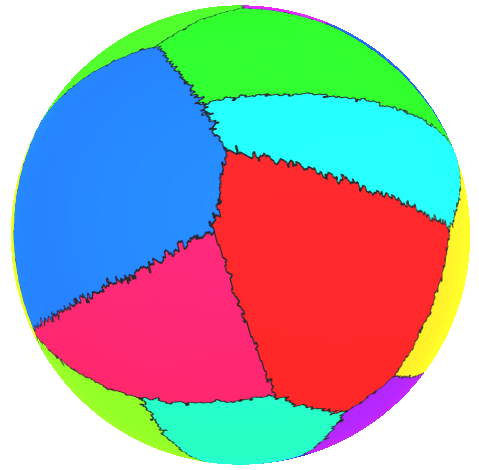
\includegraphics[height=7cm]{plate-initialization.png}
\caption{initial plates}
\label{fig:initial-plates}
\end{subfigure}
\hspace*{1cm}
\begin{subfigure}{7cm}
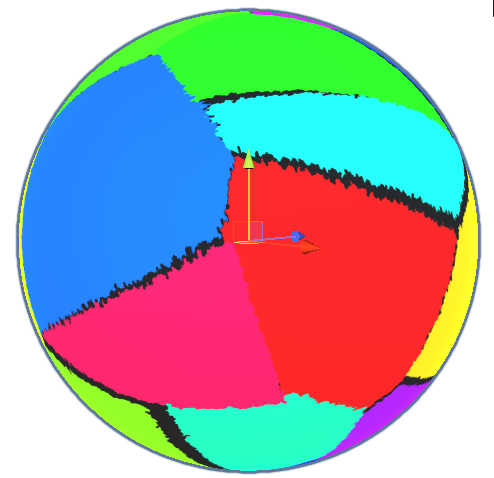
\includegraphics[height=7cm]{plate-drift.png}
\caption{plates drifting}
\label{fig:plates-drifting}
\end{subfigure}
\caption{Crust partitioning}
\label{fig:crust-partitioning}
\end{figure}
\subsection{Plate overlaps}
Tectonic interactions require the concept of plate density. For example, denser ocean plates are subducted under continental plates. Because our model does not have a clear designation of a plate as ocean or continental (any plate can have ocean or continental crust), we evaluate plates by a weighted sum of their vertices. Each plate is assigned a score equal to:
$$\mbox{score}=100\times\mbox{number of continental crust points}-\mbox{number of ocean crust points}$$
The plates are then ranked by the highest score. The rank decides which plate 'goes under' when two plates overlap (the one with a lower score). This actually creates an irreflexive, antisymmetric and transitive relation on the set of plates.

This ranking system is a gross simplification. As many simplifications, though, it makes certain decisions and calculations much easier. The plate ranks have to be recalculated every time an interaction requires them, as the scores change both with crust elevation and changes in crust point assignments to plates. An example might be when we need to know which of the overlapping plates defines a crust point elevation on the surface.
\subsection{Plate drift}
The main reason for tectonic interactions is the tectonic drift. Plates move constantly, causing collisions, subduction etc. To model the drift of a plate, during every tectonic step the plate transform is adjusted
by multiplication of the transform by a quaternion representing a rotation around the axis $\mathbf{w}$ by the angle of $\Delta\phi=\omega\delta t$. This keeps the information about current crust points locations. The result of a one step drift from the initial position can be seen in Figure \ref{fig:plates-drifting}. We can see here that the plates move as individual rigid bodies.
\subsection{Ocean crust generation \& crust resampling}
Moving rigid plates necessarily create gaps on the surface. In reality, this 'empty' space is filled with new crust drifting from ocean ridges between the plates (see Figure \ref{fig:resample-mesh}). We use the original model, only slightly simplified. We can interpolate crust data at any point on the surface which is not in any triangle belonging to a plate. We compute two distances to two nearest plates (nearest vertices belonging to two different plates) $d_1$ and $d_2$ (1 being the absolute shortest) and assume that the point is approximately on the direct line between the nearest points. We also assume that the ridge is directly in the middle of the line. This is not true in reality, but makes it simple to use the original algorithm easily. We compute the ridge and plate elevation contributions and combine them as per Cortial et al.
\begin{figure}[ht]
\centering
\begin{subfigure}{7cm}
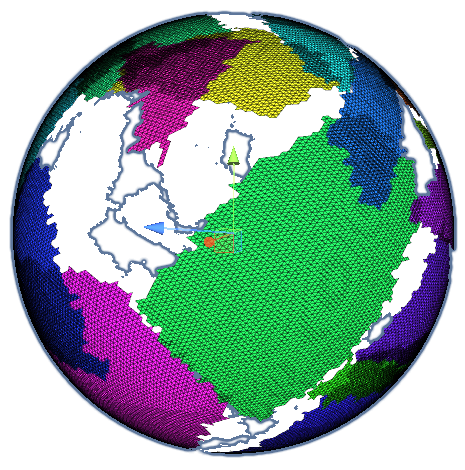
\includegraphics[height=7cm]{resample-drift.png}
\caption{diverging plates}
\label{fig:resample-drift}
\end{subfigure}
\hspace*{1cm}
\begin{subfigure}{7cm}
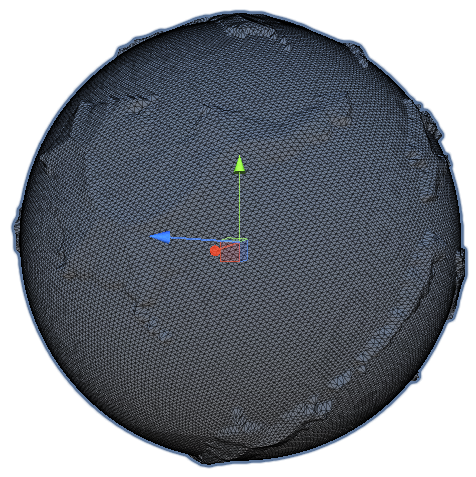
\includegraphics[height=7cm]{resample-ridges.png}
\caption{generated ridges}
\label{fig:resample-ridges}
\end{subfigure}
\caption{Ocean crust generation}
\label{fig:resample-mesh}
\end{figure}

The ridge function profile uses three parameters: the highest ocean ridge elevation $z_r$, the abyssal plains elevation $z_a$ and the ocean ridge elevation falloff $\sigma_r$. The values of these parameters are:
$$z_r=-1\mbox{ km}=-0.001\mbox{ u}$$
$$z_a=-6\mbox{ km}=-0.006\mbox{ u}$$
$$\sigma_r=0.05\mbox{ u}$$
The ridge function profile is a function of a variable $d_\Gamma$ which is the distance to the ocean ridge. The function profile is chosen as:
$$z_\Gamma=(z_r-z_a)2^{\frac{d_\Gamma}{\sigma_r}}+z_a$$
The original function profile is not specifically described and may be more complex.
Because of our assumptions we can calculate the ridge function profile variable that is the distance to the ridge as:
$$d_\Gamma=\frac{d_2-d_1}{2}$$
The orogeny type is universally filled as None for points in the surface voids. The crust age is computed as the scaling parameter $\alpha=\frac{d_\Gamma}{d_\Gamma+d_1}$ multiplied by the total time for which the plates have been diverging (since last they were in close contact). This makes the new ocean crust gradually older the further it is from the ridge. Finally, any new ocean crust point is assigned to the nearest plate.

For simulation running for many steps it is vital that we periodically resample the surface to fill the gaps made by diverging plates and to resolve overlapping plates. As per Cortial et al., it is recommended to resample the surface every 10th-60th step. Our model forces resampling on several occasions, namely continental collision. The resampling simply means to interpolate surface data onto the original mesh from the current surface data defined on a mesh broken by drifting plates and interactions. For each initial mesh vertex, we test if it is found on a plate with the highest rank possible. If so, we perform barycentric interpolation from a triangle within which the vertex currently resides. If no plate is found, we create a new ocean crust point.
\begin{table}[h]
\centering
\begin{tabular}{cccc}
\textbf{Symbol}&\textbf{Description}&\textbf{Original value}&\textbf{Model value}\\
\hline
$N$&Number of mesh vertices&-&500,000\\
$\delta t$&Tectonic time step&2 My&2 My\\
$R$&Planet radius&6,378 km&6.37 u\\
$z_{0t}$&Initial ocean elevation&-&-0.004 u\\
$z_{0c}$&Initial continental elevation&-&0.001 u\\
$e_0$&Basic crust thickness&-&0.01 u\\
$N_\mathcal{P}$&Initial number of plates&-&40\\
$p_C$&Initial continental plate probability&0.3&0\\
$v_0$&Maximum plate speed&100 mm$\cdot$y$^{-1}$&$0.0157\mbox{ My}^{-1}$\\
$n_{\mbox{sm}}$&noise averaging iterations&-&4\\
$n_{\mbox{vb}}$&Voronoi border shift iterations&-&4\\
$z_r$&Highest ocean ridge elevation&$-1\mbox{ km}$&$-0.001\mbox{ u}$\\
$z_a$&Abyssal plains elevation&-6\mbox{ km}&$-0.006\mbox{ u}$\\
$\sigma_r$&Ocean ridge elevation falloff&-&0.05\mbox{ u}\\
\end{tabular}
\caption{Model parameters summary}
\label{tab:model-parameters-summary}
\end{table}
\section{Implementation \& data model}
\label{sec:implementation}
\subsection{Project structure}
Driftworld Tectonics operates within the Unity Editor in a non-runnable scene. The basic template scene is called \asd{BasicScene}. It can be duplicated for experimenting. \asd{BasicScene} contains one critically important GameObject \asd{Planet}. A script \asd{PlanetManager} is assigned to it. \asd{PlanetManager} is a~standard MonoBehaviour script with dummy \asd{Start} and \asd{Update} methods. There is an Editor subclass \asd{PlanetEditor}, flagged as CustomEditor for \asd{PlanetManager} scripts. Because of its \asd{OnInspectorGUI} method, whenever \asd{Planet} is focused, all scene tools are available in the inspector dock.

\asd{PlanetManager} is the central script, through which all other parts interact. It keeps instances of the planet data, file management, project settings (parameters as well as assigned shaders), and a~random number generator and provides accessibility between the components. \asd{PlanetManager} is also responsible for rendering the planet through a~GameObject instance \asd{Surface}. Basic structure diagram can be seen in Figure \ref{fig:project-structure}. Arrows indicate direct access.
\begin{figure}
\centering
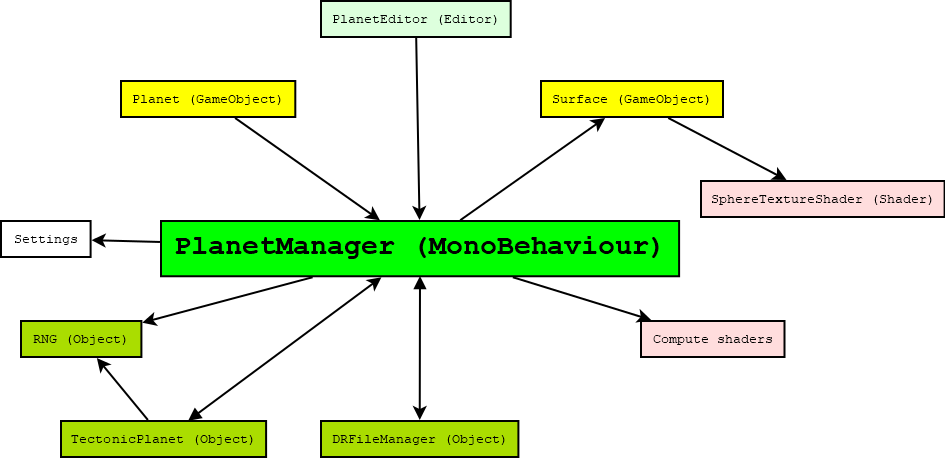
\includegraphics[width=15cm]{project-structure.png}
\caption{Simplified project structure}
\label{fig:project-structure}
\end{figure}
\subsection{TectonicPlanet object}
\asd{TectonicPlanet} is the most important data object in the project. It contains all relevant information about the simulated planet such as vertex positions, triangles, tectonic plate data, certain simulation statistics, vector noise, overlap relations and compute shader buffers. There are two main data layers, called \asd{Crust} and \asd{Data}. \asd{Crust} keeps all the tectonic model information and the simulation runs in this layer.  Because the data is interpreted as separated by plate, the layer mesh topology is broken along the plate borders. \asd{Data} layer provides compact surface data, i.~e. a~closed sphere surface mesh terrain (see Figure \ref{fig:model-layers}). Computed oceanic ridges information is only present in the \asd{Data} layer as it is not needed for plate interactions, only for resampling.
\begin{figure}[ht]
\centering
\begin{subfigure}{7cm}
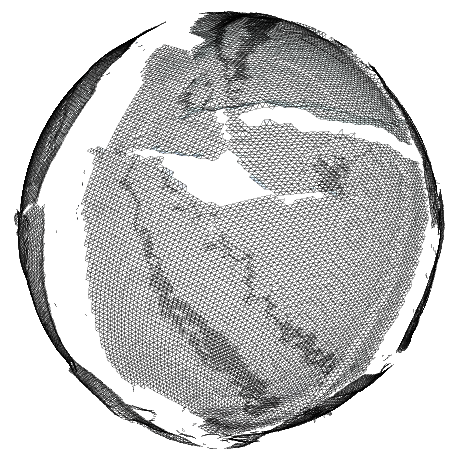
\includegraphics[height=7cm]{layer-crust.png}
\caption{crust}
\label{fig:layer-crust}
\end{subfigure}
\hspace*{1cm}
\begin{subfigure}{7cm}
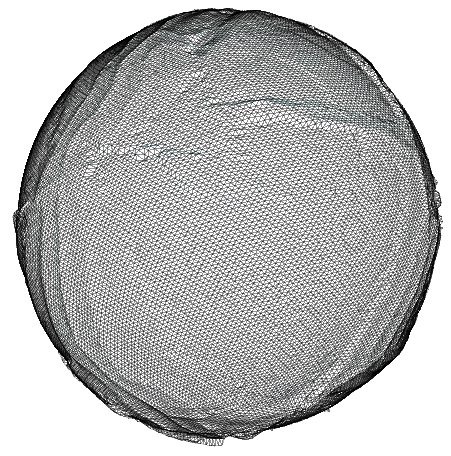
\includegraphics[height=7cm]{layer-data.png}
\caption{data}
\label{fig:layer-data}
\end{subfigure}\\
\begin{subfigure}{7cm}
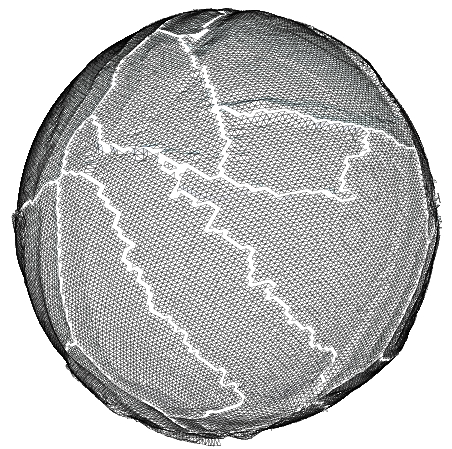
\includegraphics[height=7cm]{layer-resampled.png}
\caption{resampled crust}
\label{fig:layer-resampled}
\end{subfigure}
\caption{Model layers}
\label{fig:model-layers}
\end{figure}

Because Unity limits the number of vertices in a single mesh to the maximum UInt16 value 65,535 by default, another \asd{Render} layer is needed for rendering. It is essentially the same layer as \asd{Data}, but the information is interpolated onto a mesh with sufficiently low number of vertices.\footnote{There is a technique to render more detailed objects by splitting large meshes into chunks \cite{chunks}. In my opinion, however, this technique would add unnecessary complexity to the rendering process} The obvious problem with rendering can be seen in Figure \ref{fig:render-500k}.
\begin{figure}[ht]
\centering
\begin{subfigure}{7cm}
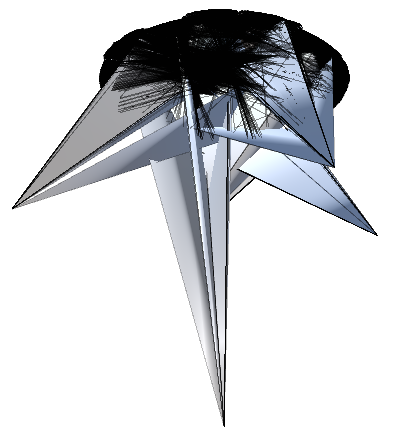
\includegraphics[height=7cm]{layer-toolarge.png}
\caption{data layer problem}
\label{fig:layer-toolarge}
\end{subfigure}
\hspace*{1cm}
\begin{subfigure}{7cm}
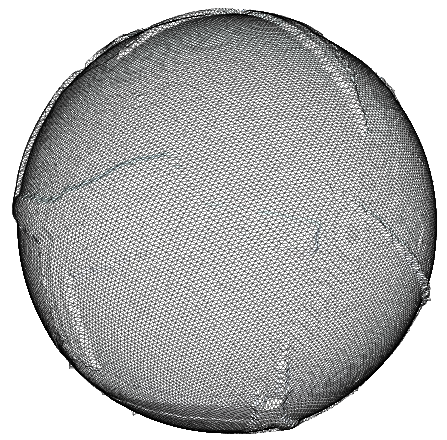
\includegraphics[height=7cm]{layer-render.png}
\caption{render layer correction at 60k vertices}
\label{fig:layer-render}
\end{subfigure}
\caption{Rendering of 500k vertices mesh}
\label{fig:render-500k}
\end{figure}
\subsubsection{Stored information}
Members of a~\asd{Planet} instance can be divided into three groups. First is the general information, including planet radius, reference to the \asd{PlanetManager} random number generator (as \asd{TectonicPlanet} heavily relies on it), vector noise data and the simulation statistics (the number of total tectonic steps performed and the number of tectonic steps performed since last resampling). The second group are the buffers needed for the compute shaders. These buffers store the planet state information in a~format suitable for GPU computing. The third group is the layer data (separately \asd{Crust}, \asd{Data} and \asd{Render}). It contains information about the vertex number and positions, the triangle number and geometry, vertex neighbours, triangle neighbours, triangles belonging to vertices, surface point data, tectonic plates and their overlap relations and the bounding volume hiearchy. Vertex positions are stored as a~list of \asd{Vector3} values, triangles are a~list of objects. Other members reference these by indexing. All members present in layers are stored separately. Description of individual layer data members follow.
\begin{itemize}[\label={}]
\item[\textbf{Vertex positions}] A~list of \asd{Vector3} type values representing positions of the samples on the unit sphere surface. These values do not change and tectonic drifts are represented by the plate quaternion transforms acting on vertex positions when needed. \asd{Crust} and \asd{Data} layer members are actually identical copies of the same information. Vertex indices point into this list.
\item[\textbf{Triangles}] A~list of \asd{DRTriangle} objects representing geometrical triangle data. Every instance has information about the vertex indices that comprise the triangle, its circumcircle, circumradius, centroid position, list of indicies of triangles sharing an edge and a~reference to the vertex position list. Again, the plate transforms are applied when needed. Triangle indices point into this list.
\item[\textbf{Vertex neighbours}] Nested \asd{int} list of indices of neighbouring vertices for each vertex (i.~e. by a~triangle edge). Index in the outer list corresponds to the index of a~vertex position.
\item[\textbf{Triangles of vertices}] Nested \asd{int} list of indices of triangles a~vertex is a~part of. vertices for each vertex (i.~e. by a~triangle edge). Index in the outer list corresponds to the index of a~vertex position.
\item[\textbf{Tectonic plates}] A~list of \asd{Plate} objects. Each instance has information about the vertices, triangles and border triangles belonging to the plate, its rotation axis, angular speed, transform, centroid position and plate-specific bounding volume hiearchy data. Plate indices point into this list.
\item[\textbf{Overlap relations}] A~two-index array antisymmetrical matrix representing the relation.
\item[\textbf{Surface point data}] A list of \asd{PointData} objects that store tectonic information: elevation, thickness, orogeny type, age and the plate index the vertex belongs to. The index in this list corresponds to the index of a~vertex position.
\item[\textbf{Bounding volume hiearchy}] Information for faster look-ups and collision tests. See subsection \ref{subsec:bvh}.
\end{itemize}

Initial data for a~new simulation are loaded from two template datafiles (their structure is described in Appendix \ref{sec:template-datafile-structure}) by the \asd{LoadDefaultTopology} method. A~template file contains the topology of a~Delaunay triangulation. One is used in the \asd{Data} layer and one in the \asd{Render} layer. No \asd{Crust} layer information is available until the simulation initializes the tectonic algorithm after some default topology is loaded.  There are several template files available with varying number of samples, but the \asd{Render} layer is limited by the maximum number of 60,000 samples.
\subsection{Bounding volume hiearchy}
\label{subsec:bvh}
During the simulation, the model performs searches in large sets of triangles many times, often for each element of another large set of vertices or triangles. Brute-force approach has the complexity of $\mathcal{O}(n^2)$. On the scale of around 100,000 elements, this adds up to $10^{10}$ iterations. Together with the fact that each iteration is not trivial to evaluate, this method is impractical. Driftworld uses bounding volume hiearches (BVH) to build a~binary search tree, reducing the total complexity to $n\log n$ \cite{sulaiman}\cite{bvharticle}.

Because the interaction space is the surface of a~unit sphere (i.~e. a~two-dimensional manifold), we choose the circumcircle as the bounding volume of a~triangle and the hiearchy is constructed from bottom up by merging circles. In \asd{Crust} layer each plate has its own BVH, \asd{Data} layer has one for the whole surface.
\subsubsection{Morton code}
Morton code is a technique which Driftworld uses to represent circle centers in an ordered manner \cite{morton}. Each circle can be assigned an \asd{UInt32} type value (synonymous to \asd{uint}) giving both coordinates inside a~grid on the sphere surface. The two spherical coordinates $\phi\in[0,2\pi)$ and $\theta\in[0,\pi]$ are normalized to intervals $\phi_1\in[0,1)$ and $\theta_1\in[0,1)$ and scaled to two \asd{UInt16} values:
$$\mbox{\asd{UInt16} }u_\phi=\lfloor 65535\phi_1\rfloor$$
$$\mbox{\asd{UInt16} }u_\theta=\lfloor 65535\theta_1\rfloor$$
The individual bits of the binary representations of $u_\phi$ and $u_\theta$ are then interlaced in a single \asd{UInt32} value $u_{\phi\theta}$ so that the least significant bit of $u_\phi$ is the least significant bit of $u_{\phi\theta}$.

\paragraph{Example} A circle has a center $\mathbf{c}(\phi,\theta)$ at (3.1,0.5). The normalized values are $\phi_1=0.493,\theta_1=0.159$. The binary representations of $u_\phi, u_\theta$ and $u_{\phi\theta}$ are:
$$u_\phi=\mbox{0111 1110 0011 010\underline{0}}$$
$$u_\theta=\mbox{0010 1000 1011 0100}$$
$$u_{\phi\theta}=\mbox{0001 1101 1101 0100 1000 1111 0011 000\underline{0}}$$
\subsubsection{Constructing BVH}
The hiearches are constructed for sets of triangles. Each triangle must provide the positions of its vertices. From this information, the circumcenters and the circumradii are calculated, which are the elementary bounding volumes. These elementary volumes become the leaves of the hiearchy tree. The construction loop begins with the merging of some suitable couples of circles, creating parent node larger circles. These new circles together with the unmerged circles become the new set of circles for the new loop iteration. The loop repeats until a single root circle is created (see Figure \ref{fig:bvh-construction}).
\begin{figure}[ht]
\centering
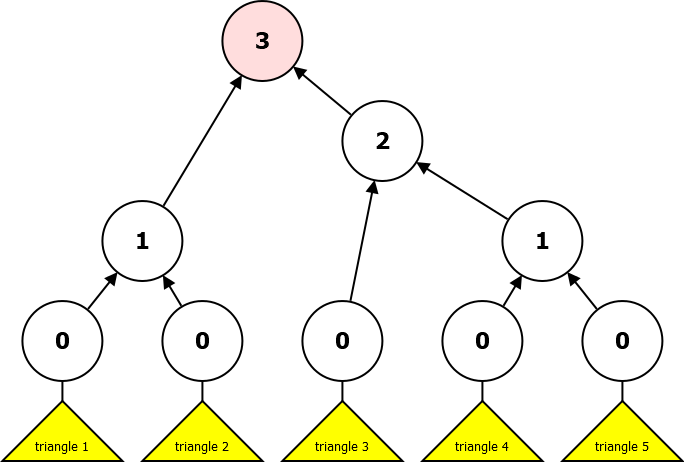
\includegraphics[width=14cm]{bvh-construction.png}
\caption{Example of a BVH construction over 5 triangles in 3 iterations}
\label{fig:bvh-construction}
\end{figure}

Merging circles randomly creates unreasonably large bounding volumes on lower levels of a BVH. It is therefore useful to identify close circles to avoid wasting space. Determining nearby clusters by brute-force has a complexity of $\mathcal{O}(n^2)$ at least, not considering cases where the nearest neighbour relation is not mutual. Because of that, Driftworld utilizes a~parallel search for suitable circle couples to be merged \cite{meister}. In each iteration, the set of circles is bucket-sorted by their Morton codes into an array. Then for each element a~candidate is selected within a range of $r_M=20$ elements (clamped to the array borders) that is the nearest and its index is flagged. If two elements are the nearest candidates of each other, their respective bounding volumes are merged for the next iteration.
\subsubsection{Searching the BVH}
Because of memory restrictions of the L1 cache of the GPU (trees are searched by compute shaders), Driftworld implements a~DFS algorithm for determining collisions or finding vertices inside triangles. The tree is searched using left-child-first rule, traversing left children first and rejecting all nodes (and their children) whose bounding volumes do not meet the collision parameters. The search stops when a colliding triangle is found or when the whole hiearchy is searched with no hit. An example of a~traversal is seen in Figure \ref{fig:dfs-traversal}. Dashed circles do not meet the collision parameters, green triangles are hits. Only the first triangle hit is considered when traversing.

The algorithm uses a~stack with the maximum size of $d_s=40$, which remembers the current path of the tree traversal.
\begin{figure}[ht]
\centering
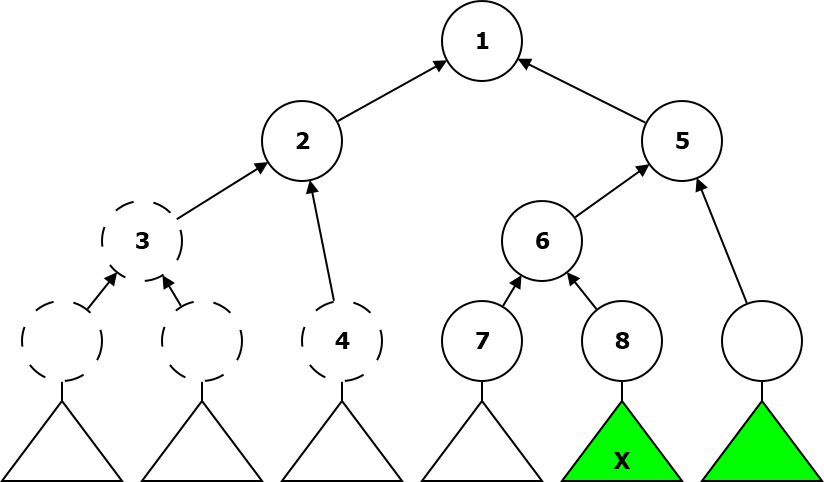
\includegraphics[width=14cm]{dfs-search-A.png}
\caption{Example of a tree traversal order}
\label{fig:dfs-traversal}
\end{figure}
\subsection{GPU Computing}
The number of processing-intensive tasks that are performed each step requires a~faster implementation using compute shaders. \asd{TectonicPlanet} stores a~dictionary of \asd{ComputeBuffer} instances. The buffers are updated only when relevant data is changed, using a~\asd{bool} dictionary for flagging. All buffers are interpreted as one-index array of either primitive types or specially designed structs understandable by the shaders. Two-dimensional arrays representing a~list of lists are accompanied by so-called sps buffer arrays with pivot points dividing individual lists. All buffers remain active in the memory unless rewritten by loading another simulation.
\begin{itemize}[\label={}]
\item[\textbf{BVH nearest neighbour shader}] Used for determining the nearest bounding volume candidates for constructing BVH. Run once per construction iteration.
\item[\textbf{Vertex data interpolation shader}]  Used for translating data between planet data layers. Interpolates point data to mesh of the correspondent layer.
\item[\textbf{Plate interactions shader}] Used for the majority of look-ups during tectonic steps.  It is the most complex shader with numerous different kernels, responsible for testing border collisions with plates, subduction uplift, continental erosion, oceanic damping, sediment accretion, slab pull contributions, contacts between continental triangles and continental collision uplift.
\item[\textbf{Overlay texture shader}] Computes pixel colors for 4096x4096 textures used in displaying data on the surface mesh.
\item[\textbf{Fractal terrain shader}] Computes changes in elevation in one fractal terrain generation iteration. This is not a~part of the Driftworld tectonic simulation.
\end{itemize}

\subsection{Precision issues}
Driftworld tools use almost exclusively \asd{float} precision because \asd{Vector3} components are of \asd{float} type and the shaders utilize FP32 cores. For the most part, 32-bit precision does not pose a problem, but sometimes certain operations suffer from rounding errors. Most notably, \asd{acos} function is used to compute distances from dot products. In some cases, a~dot product result of assumed unit vectors is greater than 1. This is obviously outside the domain of \asd{acos}, so the values are clamped to 1 manually. During BVH look-ups, the BV collisions are tested by comparing distances from the BV centers with their radii. The value of any BV radius is overestimated by 1~\% during tree traversals. This obviously decreases the efficiency of the algorithm, but also decreases the chance of a~correct BVH branch being rejected. When testing whether a point is inside a triangle, there is a tolerance of $10^{-4}$ for the results of dot products with the normals of the edge planes.

The template mesh files provide the sample position coordinates in \asd{double} precision. These need to be converted to \asd{float} when reading.
\subsection{Rendering}
\label{subsec:rendering}
Unity was chosen for this project in large part because of the ease with which data can be visualized. The \asd{Surface} GameObject is a dedicated Object in the scene used for rendering the planet surface. It can render any of the three data layers with the exception of the template mesh files with over 60,000 samples (that should be used exclusively in the \asd{Crust}/\asd{Data} layers). During rendering, the mesh takes elevation into account, despite it being separately stored in the crust point objects. The rendering has three parts: basic mesh, elevation and overlay (see subsection \ref{subsec:overlays}). The basic mesh consists of the crust vertices, which always have a~length of the planet radius $R$, and the triangles. In case of \asd{Crust} and \asd{Data} layers all triangles of the surface mesh are fed to the \asd{MeshFilter} component. The \asd{Crust} layer only considers triangles that are entirely a part of a tectonic plate. This is because triangles between plates have distorted geometry due to the plate transforms. The elevation part is used for adjusting the length of mesh vertices to visualize surface details. Any unit vertex $\mathbf{u}_i$ on the surface has an accompanying elevation value $z_i$. The actual vertex that is fed to the \asd{MeshFilter} is:
$$\mathbf{u}_i'=(R+h_ez_i)\mathbf{u}_i$$
$h_e=50$ is the elevation scale factor used for stressing the surface features. The vertices are fed through an array of \asd{Vector3} values and the triangles are a~one-dimensional sequential array of triples of indices within the vertex array.

Figure \ref{fig:render-layers} shows examples of renders of the same simulation state in different layers. Faults in the plate topology are clearly seen in Figure \ref{fig:render-crust}. Figure \ref{fig:render-data} shows full \asd{Data} layer mesh with prominent surface features. The relative decrease in the \asd{Render} layer mesh resolution is shown in Figure \ref{fig:render-normal}, although since the overlays are computed at the \asd{Data layer}, some details are preserved in the texture. Setting the elevation scale to 1 (true relative scale) reveals how the terrain has very little influence on the apparent surface from distance (Figure \ref{fig:render-escale1}).

User can choose to clamp the render to the ocean level, hiding all surface details below the ocean level. The ocean would appear as somewhat spherical portion of the planet.

\begin{figure}[ht]
\centering
\begin{subfigure}{7cm}
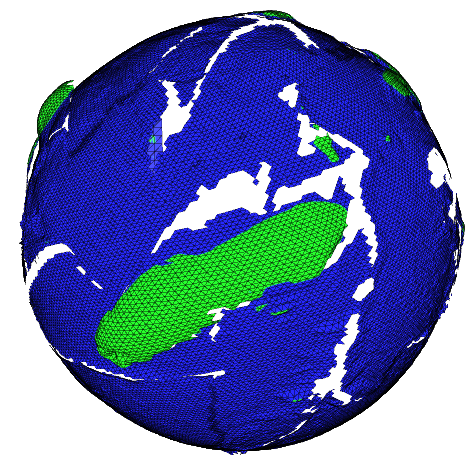
\includegraphics[height=7cm]{render-crust.png}
\caption{crust layer at 60,000 samples}
\label{fig:render-crust}
\end{subfigure}
\hspace*{1cm}
\begin{subfigure}{7cm}
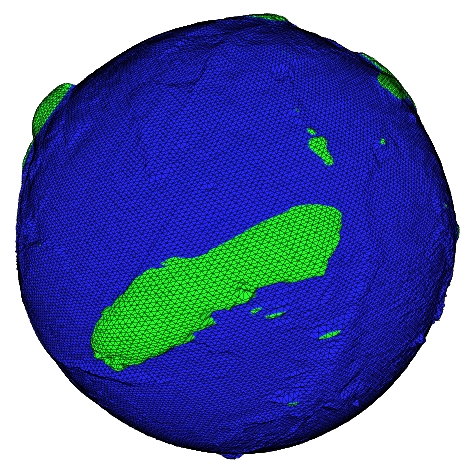
\includegraphics[height=7cm]{render-data.png}
\caption{data layer at 60,000 samples}
\label{fig:render-data}
\end{subfigure}\\
\begin{subfigure}{7cm}
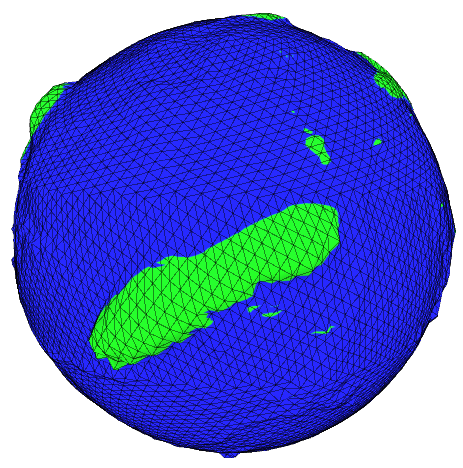
\includegraphics[height=7cm]{render-normal.png}
\caption{render layer at 10,000 samples}
\label{fig:render-normal}
\end{subfigure}
\hspace*{1cm}
\begin{subfigure}{7cm}
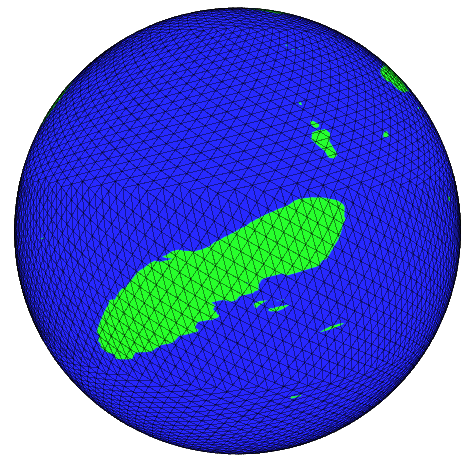
\includegraphics[height=7cm]{render-escale1.png}
\caption{render layer with elevation scale 1}
\label{fig:render-escale1}
\end{subfigure}
\caption{Renders with the basic terrain overlay}
\label{fig:render-layers}
\end{figure}
\subsection{Overlays}
\label{subsec:overlays}
Overlay is a \asd{Texture2D} image assigned to the \asd{Renderer} component \asd{\_MainTex} property of the \asd{Surface} GameObject. Any overlay is computed by the Overlay texture compute shader on-the-fly before assignment. There is a~number of different overlays implemented for checking the state of the simulation. The user can select between them independently of the layer chosen. The render does not require an overlay, leaving the object with the basic white albedo. Figure \ref{fig:overlay-render} shows examples of overlay renders with the same simulation state as Figure \ref{fig:render-layers}. Texture pixels use barycentric interpolation.
\begin{figure}[ht]
\centering
\begin{subfigure}{4cm}
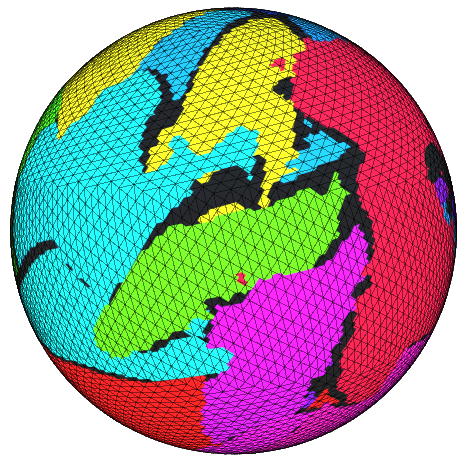
\includegraphics[height=4cm]{overlay-crustplates.png}
\caption{crust plates}
\label{fig:overlay-crustplates}
\end{subfigure}
\hspace*{1cm}
\begin{subfigure}{4cm}
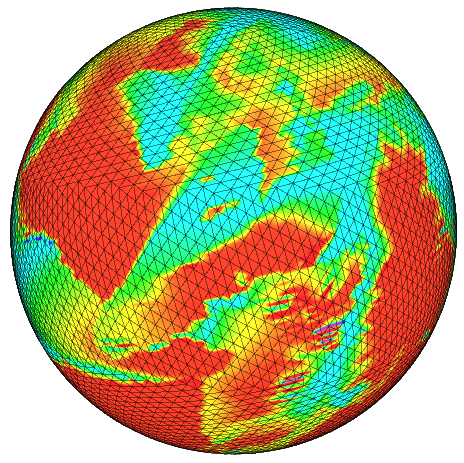
\includegraphics[height=4cm]{overlay-crustage.png}
\caption{crust age}
\label{fig:overlay-crustage}
\end{subfigure}
\hspace*{1cm}
\begin{subfigure}{4cm}
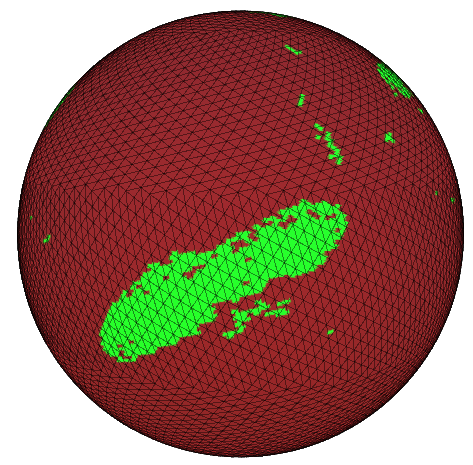
\includegraphics[height=4cm]{overlay-orogeny.png}
\caption{orogeny}
\label{fig:overlay-orogeny}
\end{subfigure}\\
\begin{subfigure}{4cm}
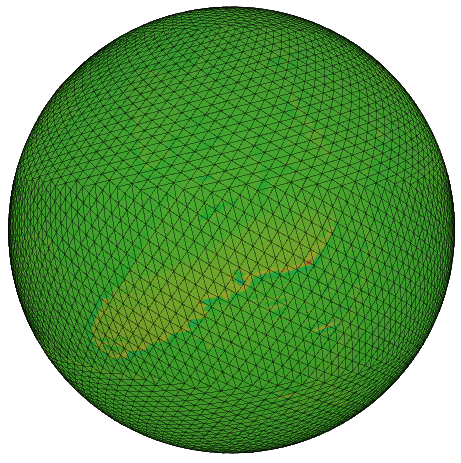
\includegraphics[height=4cm]{overlay-elevationlaplacian.png}
\caption{elevation Laplacian}
\label{fig:overlay-elevationlaplacian}
\end{subfigure}
\hspace*{1cm}
\begin{subfigure}{4cm}
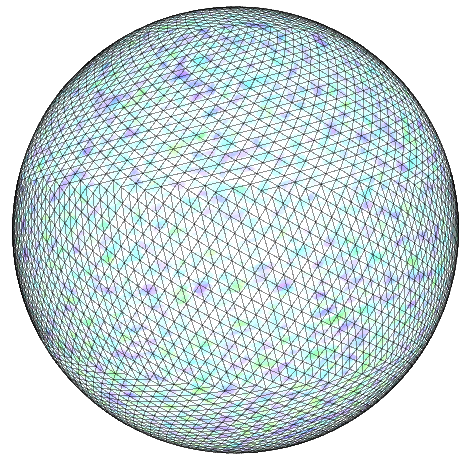
\includegraphics[height=4cm]{overlay-vectornoise.png}
\caption{vector noise}
\label{fig:overlay-vectornoise}
\end{subfigure}
\hspace*{1cm}
\begin{subfigure}{4cm}
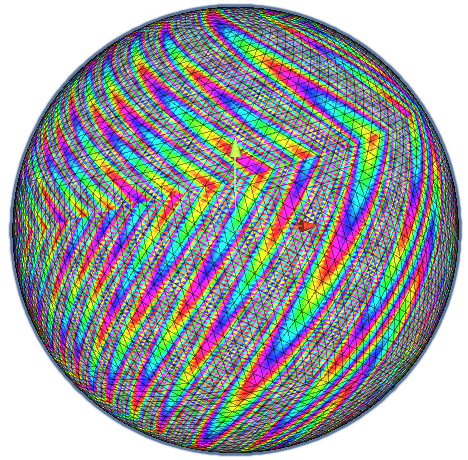
\includegraphics[height=4cm]{overlay-debugdatatriangles.png}
\caption{debug triangles}
\label{fig:overlay-debugtriangles}
\end{subfigure}\\
\caption{Overlay examples}
\label{fig:overlay-render}
\end{figure}
\begin{itemize}[\label={}]
\item[\textbf{Basic terrain}] This is the primary overlay. It is a simplified texture, differentiating between crust points below and above the ocean level. Points below the ocean level (zero elevation) have blue pixels, green otherwise. There is an error state overlay, such as when missing data for computing a~texture. It is a~solid bright red overlay.
\item[\textbf{Crust plates}] Domains of individual tectonic plates are shown. They are distinguished by the color hue.
\item[\textbf{Crust age}] Colors represent relative crust age. Red hue is for the oldest crust, blue for the newest near the oceanic ridges. Hue increases on a~standard color wheel.
\item[\textbf{Orogeny}] Three colors distinguish between different orogenies. Dark red is of None type, green is for Andean, blue for Himalayan.
\item[\textbf{Elevation Laplacian}] Used for detecting large slopes in elevation. Green is for relatively flat mesh, redder are for peaks.
\item[\textbf{Vector noise}] The representation of the simulation vector noise. Hue determines relative direction, saturation the intensity of the noise.
\item[\textbf{Debug data triangles}] Individual triangles in the \asd{Data} layer are painted in different hues. Mesh triangle ordering patterns are visible.
\item[\textbf{Debug crust triangles}] The same as for data triangles, although in the \asd{Crust} layer. Points between plates are painted black like the door.
\end{itemize}
\subsection{No amplification}
At the present state the amplification methods discussed by Cortial et al. are not implemented. Subsequent processing is possible for the saved simulations. This, however, requires interpolating the data onto a finer mesh. A~first-person agent would percieve the surface as nearly flat. The simplest method for enhancing the simulated surface could be a multi-frequency Perlin noise. Lack of an~amplified terrain should not seriously alter simulations such as hydrosphere.
\subsection{Random number generator}
Random numbers are used for initializing plates, creating vector noise, rifting events, safeguarding precision error cases and creating a~reference random fractal terrain. Standard linear congruential generators are insufficient for any advanced simulations, so Driftworld uses an implementation of a~Mersenne Twister. The implementation code is adapted from a~website example by PROWAREtech \cite{prowaretech}.

There is a single instance of the generator to assure consistent results. The state can be reset by providing a~seed parameter. The state of the generator is saved along the data when saving the simulation state to a~file.
\subsection{Use}
User has relatively large control over different aspects of the simulation. All model parameters can be changed in the inspector even between steps. The inspector controls show a~degree of accessibility logic, such as not being able to perform tectonic steps without initialized plates etc.

The inspector has several sections. First are the basic settings. Template data filenames for the \asd{Data} and \asd{Render} layers are the files that are read when loading a~fresh new simulation. Save filename is used to store ongoing simulation. The texture save filename is for saving any overlays as a~PNG image. The random number generator seed is for initializing the Mersenne Twister either before starting a~new simulation or between tectonic steps. The number of tectonic steps are performed in sequence per one activation. Lastly, the elevation scale factor was discussed in subsection \ref{subsec:rendering}.

\asd{PlanetManager} keeps an instance of two serializable sets of settings. The main settings collection  keeps all model parameters and other too, such as the Morton array look-up radius $r_M$. The shader settings are used to assign shader files. These are referenced whenever a kernel dispatch is to be called.

The overview section in the inspector shows some basic information about the simulation state. If a~loaded planet simulation is present, the overview shows the number of vertices and triangles both in \asd{Data} and \asd{Render} layer. Current rendering mode is displayed, although the user can check it in the render options. Current number of tectonic plates is important for fine-tuning the rifting frequency. Simulation statistics show the total number of tectonic steps taken and the number of tectonic steps taken without resampling.

A~fresh new simulation is loaded by the \asd{Load new planet} button. Correct filenames must be provided in the settings or the default topology load will fail. When an instance of \asd{TectonicPlanet} is active, it is possible to save the state by the \asd{Save planet to file} button. \asd{Load planet from file} overwrites any current simulation by loading a~saved simulation state from a~file. Correct filename must be provided. Note that rewriting the current simulation by any other, as well as changing a~script code (and forcing Unity to recompile) voids the current compute buffers. These must be cleared before changing the simulation in this way.

Render options are a~set of tools to look at different aspects of the simulation. User can choose an overlay or a~layer to render. Several switches control if the data should be automatically interpolated onto higher levels when needed (\asd{Crust} $\rightarrow$ \asd{Data} $\rightarrow$ \asd{Render}), if the render is clamped to the ocean level or whether the overlays should be painted over the rendered object or not. \asd{Wash texture} removes any overlay currently displayed and \asd{Render surface} renders the object with any new settings without performing a~tectonic step.

Tectonic tools are the main controls of the simulation. \asd{Initialize tectonic plates} creates a new random tectonic configuration (it a actually starts a~new simulation on a~loaded mesh). This allows for the tectonic steps to be performed. Any part of the tectonic simulation can be switched for fine-tuning or adjusting the simulation. \asd{Resample crust} manually forces resampling of \asd{Crust} layer data. Tectonic step is the manual activation tool to perform a~sequence of tectonic steps set above (1 is recommended for purposes other than fine-tuning). Calling for plates initialization requires clearing the buffers.

Data manipulation has several tools to help adjust the simulation. Clearing the buffers is the most important if the user wants to load another simulation or make changes to the script code. Smoothing elevation flattens the terrain by neighbour elevation averaging. It uses a~\textit{neighbour smooth} parameter $z_s=0.1$ , which represents the weight of the neighbour elevation when averaging. Laplacian smooth elevation performs a~similar action, however the weights are differences in elevation scaled to the maximum elevation range. RNG initialization resets the random number generator to the state denoted by a~set seed. Calculating thickness is a~placeholder action that recalculates the default thickness (this crust point information is not implemented in a~contextual manner). Forcing a~plate rift creates two new randomly divided plates from the largest plate in the \asd{Crust} layer. User can export an~overlay texture at any time, provided there is one rendered.

There is the possibility of creating a~standard fractal terrain. This does not simulate orogeny, crust age or other aspects of the tectonic simulation. It takes place entirely within the \asd{Data} layer. There are two main parameters that drive the fractal terrain generation: fractal terrain elevation step $z_f=0.003\mbox{ u}$ and fractal terrain iterations $n_f=10,000$. It runs in a~loop of $n_f$ iterations.  Each iteration chooses a~random plane passing the origin and changes elevation of every \asd{Data} point by $z_f$ -- increases on one side of the plane, decreases on the other. Data from fractal terrain generation can be used to a~degree, but the user must keep in mind that only elevation values are created. For quicker computation, fractal terrain generation uses a~dedicated compute shader and the random normal vectors of the planes are provided beforehand to the dispatched kernel. The elevations are computed for each point independently (one thread -- one vertex). Also note that the parameters $z_f$ and $n_f$ depend on each other.

Diagnostic tools are used to check the sanity of the topology and elevation. \asd{BVH Diagnostics} checks the bounding volume hiearchies for both \asd{Crust} and \asd{Data} layers, showing basic information about the look-up trees. The most relevant information is the tree depth, because a healthy tree should have a~depth of around $\log_2n$, where $n$ is the number of triangles in the hiearchy. \asd{Mesh and elevation value diagnostics} checks the sanity of the mesh. Vertex magnitude is evaluated (should be 1 within tolerance of 0.0001) and the elevation values must not have a \asd{NaN} or some infinity value. All layers are checked.

There is a~group of four work-in-progress tools that are blank. Their code can be adjusted for debugging or trying new things. They have a~wide access to all simulation data.
\begin{table}[h]
\centering
\begin{tabular}{ccc}
\textbf{Symbol}&\textbf{Description}&\textbf{Value}\\
\hline
$r_M$&Morton array look-up radius&20\\
$d_s$&Maximum stack size for DFS search&40\\
-&Bounding volume radius tolerance&1 \%\\
-&Triangle interior test tolerance&$10^{-4}$\\
$h_e$&Elevation scale factor&50\\
$z_s$&Neighbour smooth parameter&0.1\\
$z_f$&Fractal terrain elevation step&0.003\mbox{ u}\\
$n_f$&Fractal terrain iterations&10,000\\
\end{tabular}
\caption{Implementation parameters summary}
\label{tab:implementation-parameters-summary}
\end{table}
\section{Performance \& problems}
\label{sec:performance}

\section{Conclusion}
\label{sec:conclusion}
The promise of Driftworld Tectonics is to create interesting planet surfaces either for rendering or further development -- a~goal which I believe it has achieved. The simulations loosely follow tectonic processes present on Earth. Since the project is an attempted implementation of the broadly described tectonic method of Cortial et al., it should provide similar features and advantages. Indeed, many of the features seem to be present (at least in my opinion). However, it should be noted that the work presented by Cortial et al. is much more sophisticated. Driftworld Tectonics, however, offers a~detailed description of its every aspect, which may inspire further improvements, optimizations and extensions. The project is meant to be as modular as possible so that changes would not break the project structure too badly.

The lack of terrain amplification is intentional to keep the project somewhat simple. All relevant data is available in the output files, so any subsequent amplification procedure may take place. It stands to reason that folding direction should be implemented in this stage of simulation -- hopefully, this will soon be the case.

There is still much work to be done. Issues that have come up during the development of Driftworld need to be addressed so that any simulation can be reliable and smoothly operating.

It is my hope that this project inspires content creators and developers to either improve on present tectonic approximation projects or make use of Driftworld Tectonics or other available software to create worlds and stories told on these worlds.
\subsection{Continuation of work}
Driftworld Tectonics is only the first step. The real ambition is to create rich worlds with water, weather, winter or spring, plants and animals, and ultimately, people. Each part of this ambition is a~huge project on its own, it has different requirements, different ideas and approaches. At this moment, I can hardly imagine the complexity of these projects and how monumental the effort will be to undertake them. I do believe that every part of this ambition has some value on its own.

For the immediate future, a~climate model should be created on the simulation output. Calculating heat distribution during a year and the hydrosphere model seems like a logical next step. Then, amplification of the terrain is necessary to obtain any kind of presentable planet.

Any notion of a~biosphere depends on the previous steps and in turn, influences both the climate and the hydrosphere as a~whole. A~stable model should follow where deserts have a~reason and forests do not thrive without rain. The goal is not to create true simulations but to bring believable biomes.

The final step -- people. This unfortunately seems so far that all ambition -- culture, language, history, agriculture, war or infrastructure -- is a~vague, shapeless dream, so far only in the imagination of a~writer. Maybe after a~few years, some parts of this ambition will take more solid shape so that anyone can be surprised to hear an exotic language spoken on a~tropical island in the middle of an ocean.
\newpage
\begin{thebibliography}{9}
\bibitem{cortial}
Cortial, Y., Peytavie, A., Galin, E. and Guérin, E. (2019), Procedural Tectonic Planets. \textit{Computer Graphics Forum}, 38: 1-11. https://doi.org/10.1111/cgf.13614
\bibitem{meister}
D. Meister and J. Bittner, "Parallel Locally-Ordered Clustering for Bounding Volume Hierarchy Construction," in \textit{IEEE Transactions on Visualization and Computer Graphics}, vol. 24, no. 3, pp. 1345-1353, 1 March 2018, doi: 10.1109/TVCG.2017.2669983.
\bibitem{generatedgames}
Wikipedia contributors. (2022, March 20). List of games using procedural generation. In \textit{Wikipedia, The Free Encyclopedia}. Retrieved 06:20, May 19, 2022, from \url{https://en.wikipedia.org/w/index.php?title=List\_of\_games\_using\_procedural\_generation\&oldid=1078237416}
\bibitem{daggerfall}
Brogan, J. (2016, October 5). \textit{The Daggerfall Paradox}. SLATE. Retrieved May 19, 2022, from\\ \url{https://slate.com/technology/2016/10/the-paradox-of-procedurally-generated-video-games.html}
\bibitem{augustus}
Keriew, \textit{Augustus}, (2021), GitHub repository, \url{https://github.com/Keriew/augustus}
\bibitem{rimworld}
Game Developer Conference [GDC]. (2019). \textit{RimWorld: Contrarian, Ridiculous, and Impossible Game Design Methods} [Video]. YouTube. https://www.youtube.com/watch?v=VdqhHKjepiE
\bibitem{palmer}
Palmer, C. I., \& Leigh, C. W. (1934). \textit{Plane and spherical trigonometry}. New York: McGraw-Hill Book Company, Inc. 
\bibitem{keinert}
Keinert, Benjamin  \& Innmann, Matthias \& Sänger, Michael \& Stamminger, Marc. (2015). Spherical Fibonacci Mapping. \textit{ACM Transactions on Graphics}. 34. 1-7. 10.1145/2816795.2818131. 
\bibitem{todhunter}
Todhunter, Isaac. (1886). \textit{Spherical Trigonometry: For the Use of Colleges and Schools} (5th ed.). London: Macmillan and Co.
\bibitem{scratchapixel}
\textit{Ray Tracing: Rendering a triangle}. Scratchapixel 2.0. Retrieved June 6, 2022, from \url{https://www.scratchapixel.com/lessons/3d-basic-rendering/ray-tracing-rendering-a-triangle/barycentric-coordinates }
\bibitem{voronoi}
Pokojski, Wojciech \& Pokojska, Paulina. (2018). Voronoi diagrams – inventor, method, applications. \textit{Polish Cartographical Review}. 50. 141-150. 10.2478/pcr-2018-0009. 
\bibitem{delaunay}
 Delaunay, Boris. (1934). Sur la sphere vide. A la memoire de Georges Voronoi. \textit{Bulletin de l’Academie des Sciences de l’URSS. Classe des sciences mathematiques et naturelles}, Issue 6, pp. 793–800.
 \bibitem{knuth}
 Guibas, L. J., Knuth, D. E., \& Sharir, M. (1992). Randomized incremental construction of Delaunay and Voronoi diagrams. \textit{Algorithmica}, 7(1-6), 381–413. doi:10.1007/bf01758770 
 \bibitem{ma}
Ma,  Yingdong \& Chen, Qian. (2010). Fast Delaunay Triangulation and Voronoi Diagram Generation on the Sphere. \textit{2010 Second World Congress on Software Engineering},  pp. 187-190, doi: 10.1109/WCSE.2010.136
\end{thebibliography}
\newpage
\listoffigures
\listoftables
\newpage
\appendix
\section{Project parameters}
\label{sec:projectparameters}


\end{document}
